\documentclass[11pt,letterpaper]{article}
\input{headings}
\newcommand \recipeName {Oats Country Cake}
\newcommand \fileName {BoloCaipiraComAveia}
\chead{\recipeName}

\begin{document}
\input{title}


My mother made this cake when we were visiting my brother in Bras\'ilia. It was very good and I asked for the recipe. Many variations are possible. To make it gluten-free see note on powdering the oats to coat the pan. For a version without milk, substitute almond milk for milk --- usually people with lactose intolerance may consume parmesan cheese. For a vegetarian  version use sun-dried tomatoes preserved in oil in place of chicken. For a piscitarian recipe use tuna. For a sinful recipe use   fried bacon instead of chicken and add 1/2 cup of cubed gruyere or sharp cheddar cheese.
 
\begin {description}

\item [Ingredients:] \ \\
\begin {itemize}
\item 1 cup rolled oats (100 grams)
\item 1 can of corn (200 grams) at room temperature
\item 4 eggs
\item 1/4 cup canola oil (50 ml)
\item 1 cup milk (250 ml)
\item 1 teaspoon salt
\item 1/2 tablespoon dried oregano
\item 1 cup of green green onions and parsley chopped
\item 50 grams of grated parmesan
\item 1 tablespoon baking powder
\item 100 grams of chicken breast cooked with salt and shredded 
\item 2 Italian diced tomatoes (220gr)
\item Oil and flour to grease and flour the shape
\end {itemize}

\item [Procedure:] \ \\
\begin {enumerate}
\item {\bf Preheat oven and prepare form.}
\begin {itemize}
\item Turn the oven to 200 C.
\item Oil the shape very well with oil
\item Spray very well with the bread flour. For a gluten-free version, put two tablespoons of oatmeal on the food processor and process to obtain a flour. Pulverize the pan with this flour instead of the bread crumbs. 
\end {itemize}


\item {\bf Process the Oats}
\begin {itemize}
\item Put the oats in the bowl of the food processor and pulse five or six times until you obtain coarse flakes.
\item Dump the flakes in  large bowl.
\end {itemize}

\item {\bf Process wet ingredients}
\begin {itemize}
\item In a food processor or blender, process the eggs, corn, oil, milk and salt until a homogeneous mass is obtained.
\item         Transfer the mixture to the bowl that contain the oat flakes.
\end {itemize}
\item {\bf Add the dry ingredients}
\begin {itemize}
\item Add the oregano, the green onions and parsley, the oats, the parmes \~ to the grated and the yeast and mix.
\item Add chicken and tomatoes, or tuna, or dried tomatoes (if using dry tomatoes, do not use fresh tomatoes).
\end {itemize}
\item {\bf Bake}
\begin {itemize}
\item Place the mixture in the pan and bake in preheated oven (200 C) and bake for approximately 40 minutes.
\item The cake is baked when a toothpick inserted in the center comes out clean.
\item Remove from the oven and let it cool for 5 minutes.
\item Thread a narrow tip knife around the shape and around the center.
\item Place the serving dish on top of the shape and invert the shape to unmold the cake.
\item Serve warm.
	\end{itemize}
	\end{enumerate}
\end{description}

\begin{table}
\begin{tabular}{cccc}
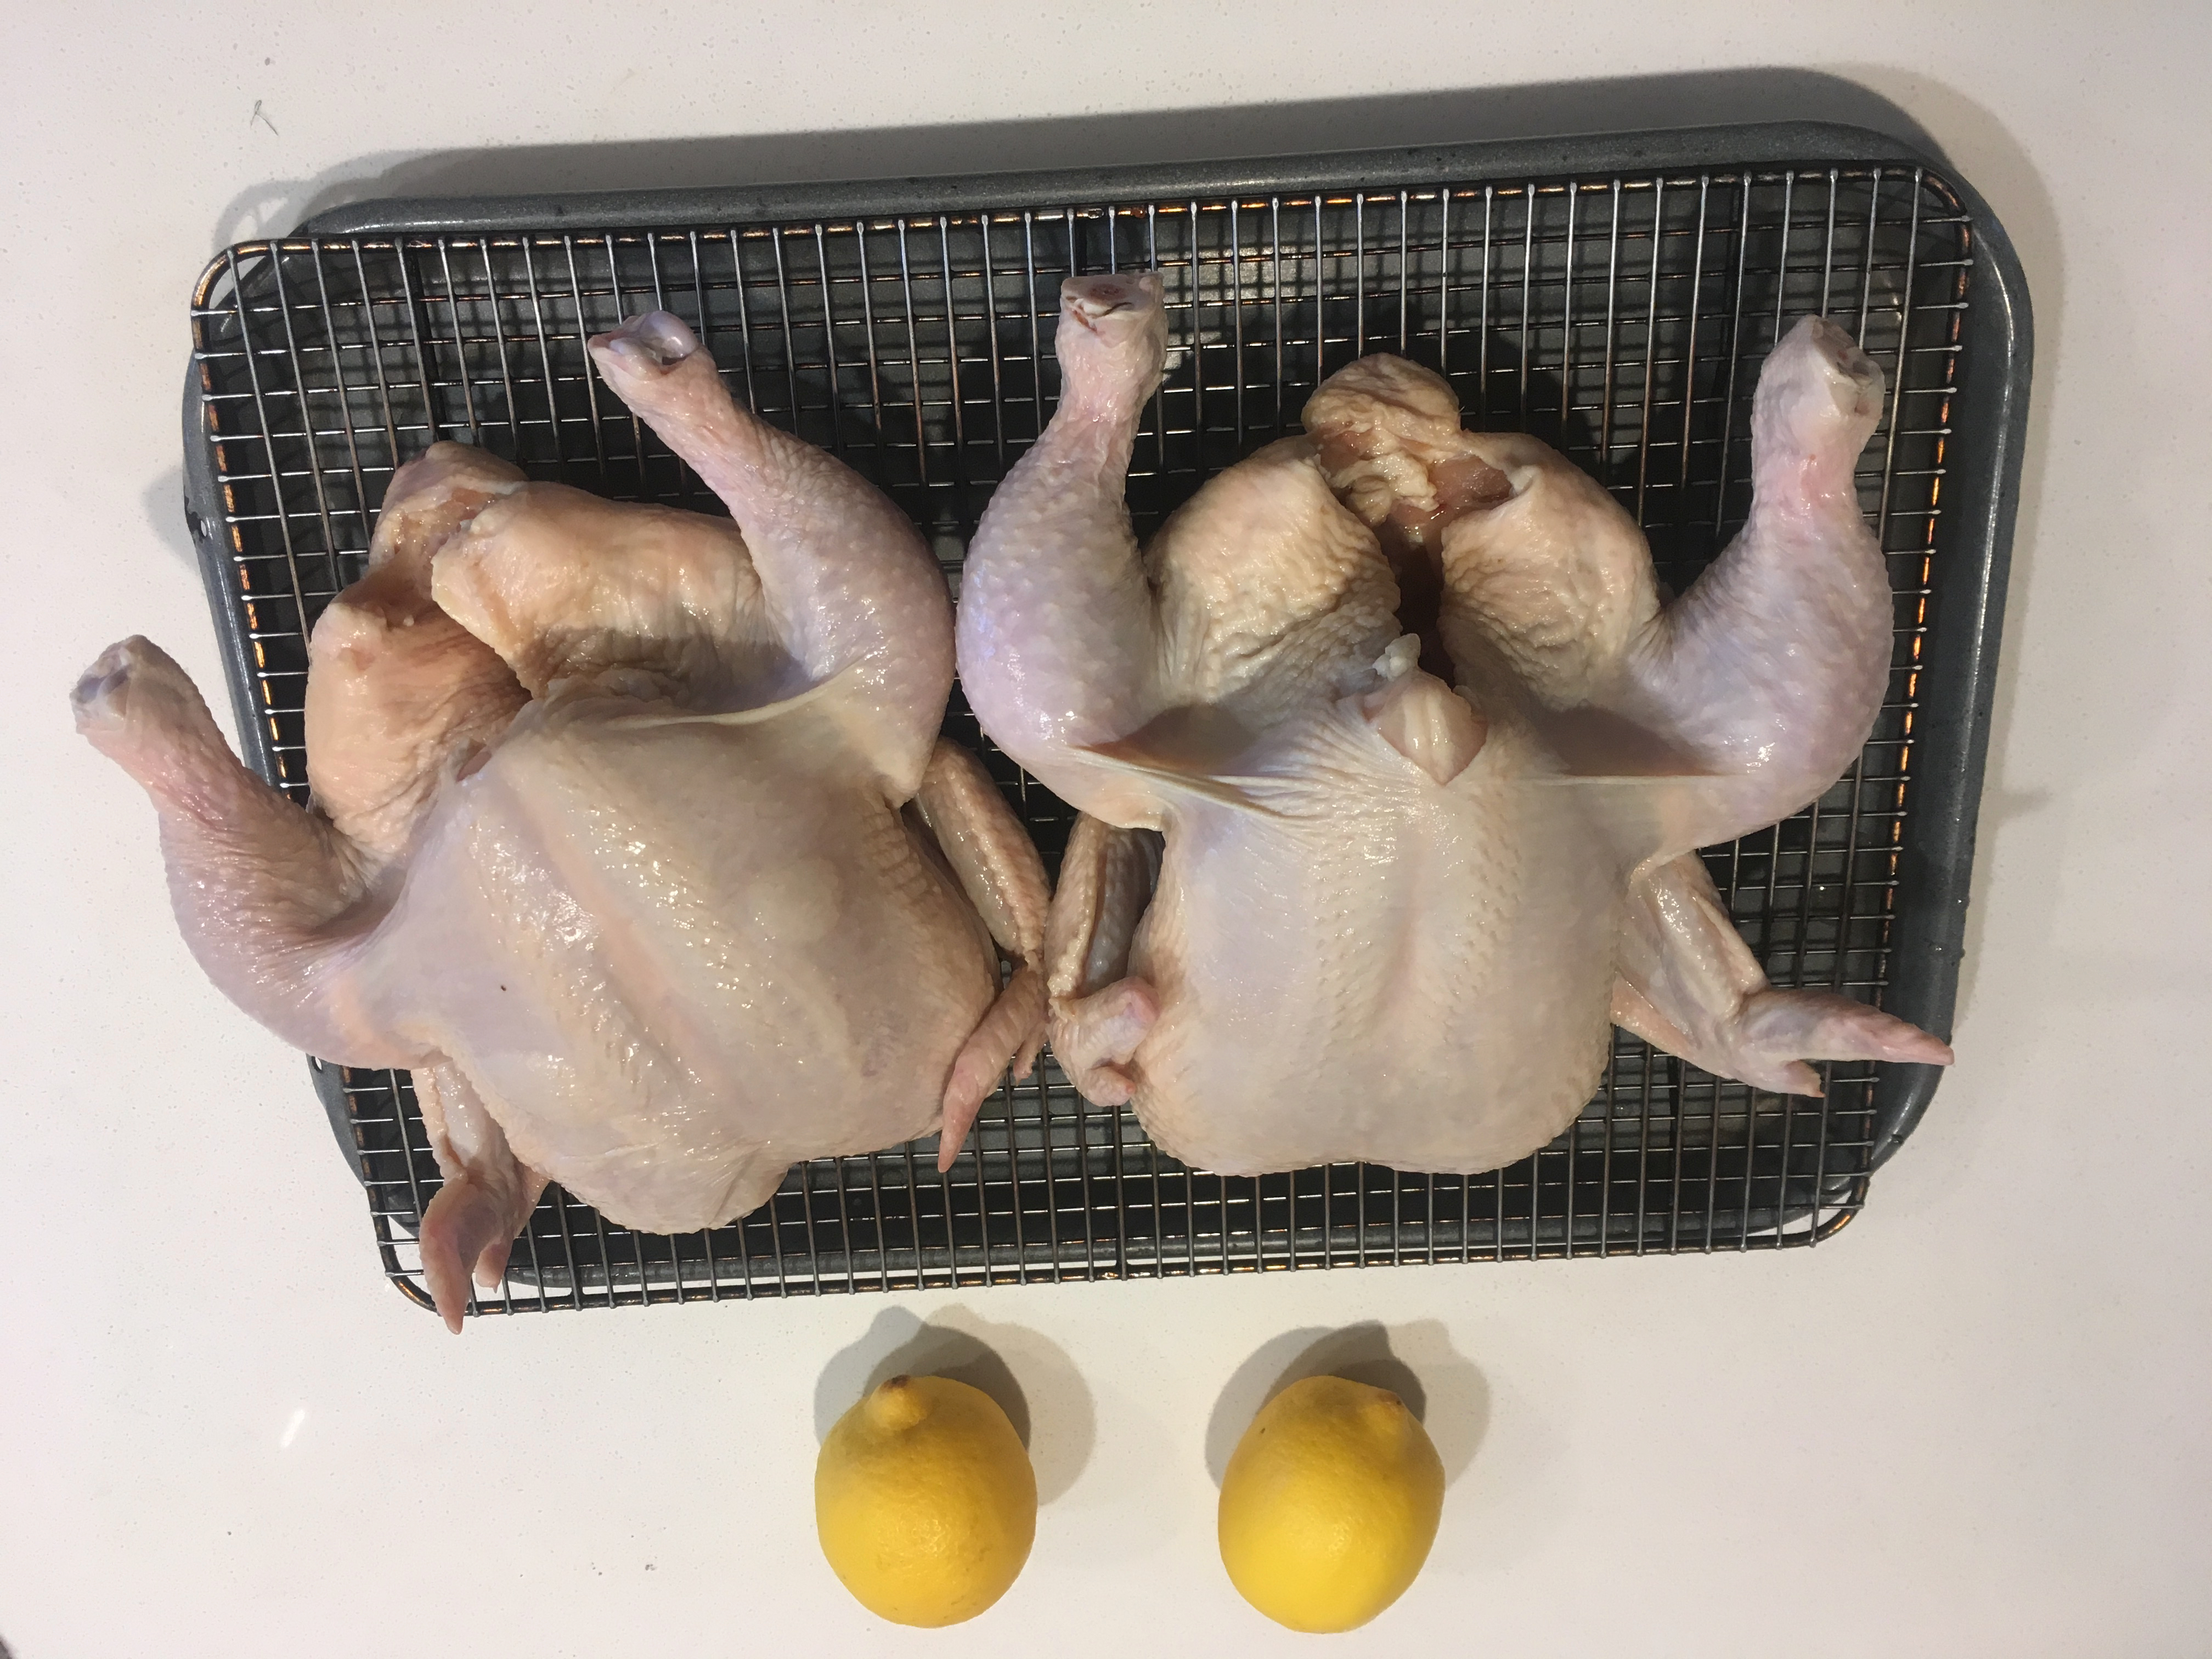
\includegraphics[width=0.25\textwidth]{\imageDir/\fileName/IMG_3197.jpg} &
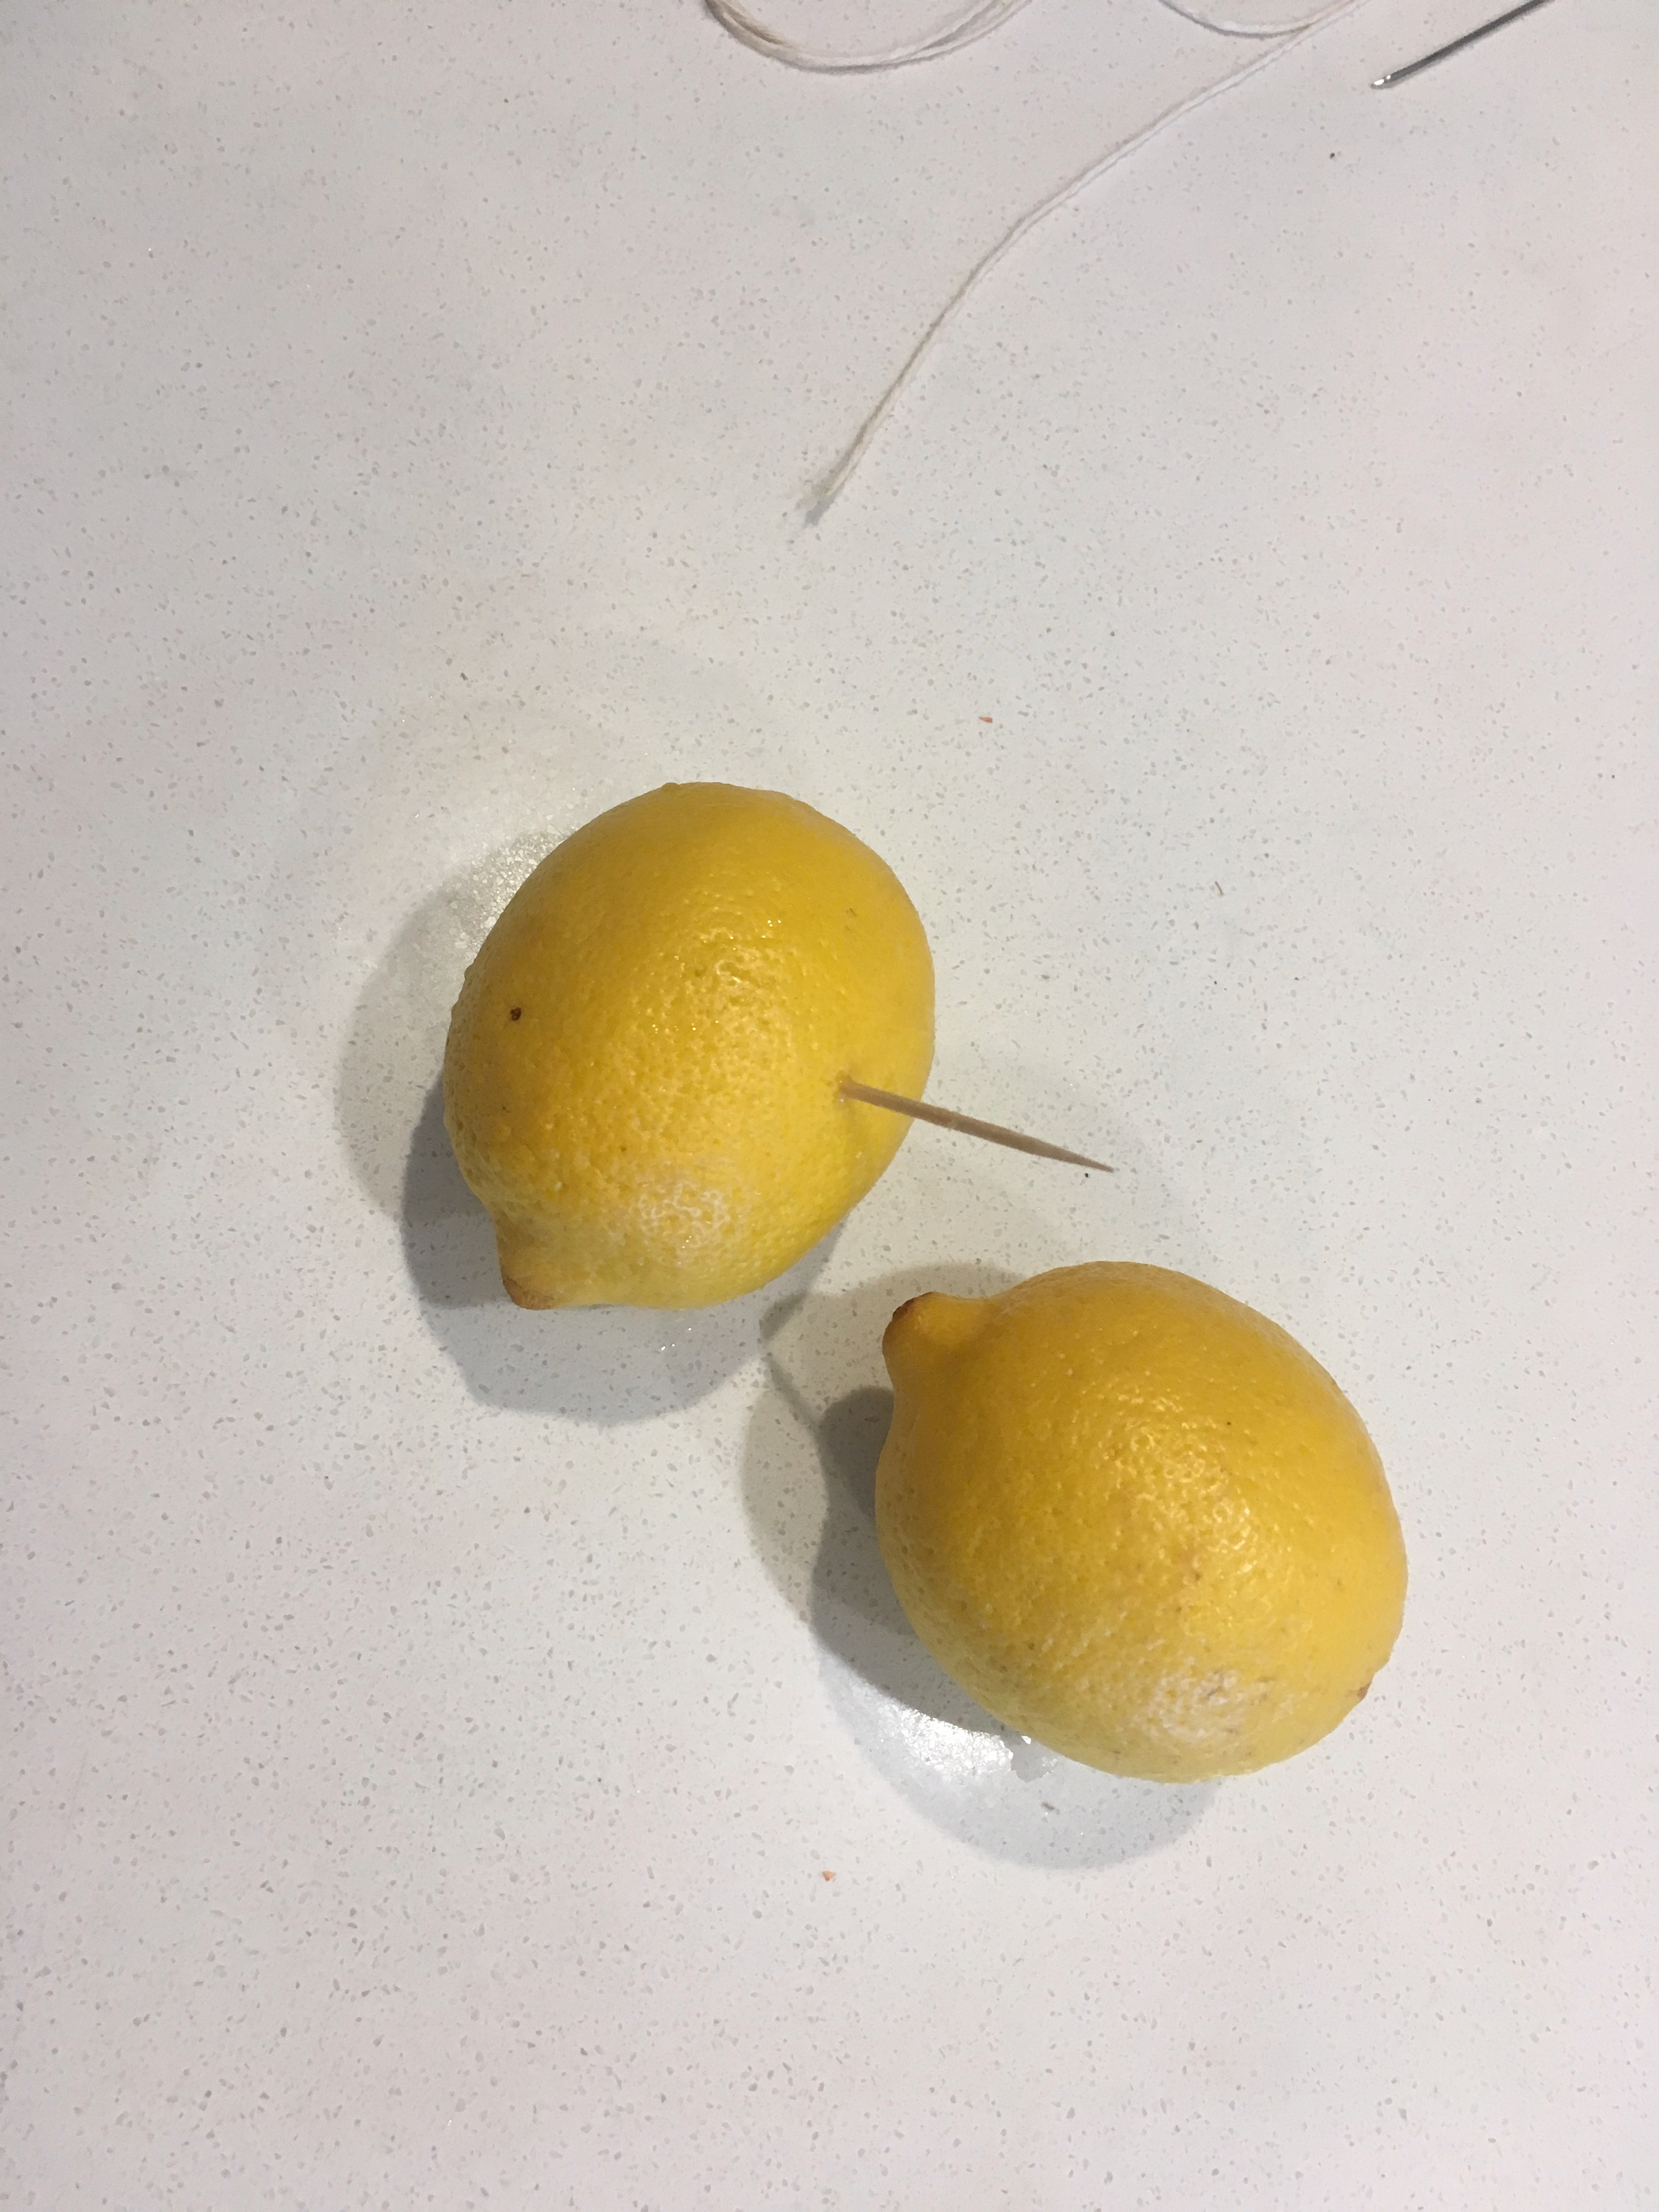
\includegraphics[width=0.25\textwidth]{\imageDir/\fileName/IMG_3212.jpg} &
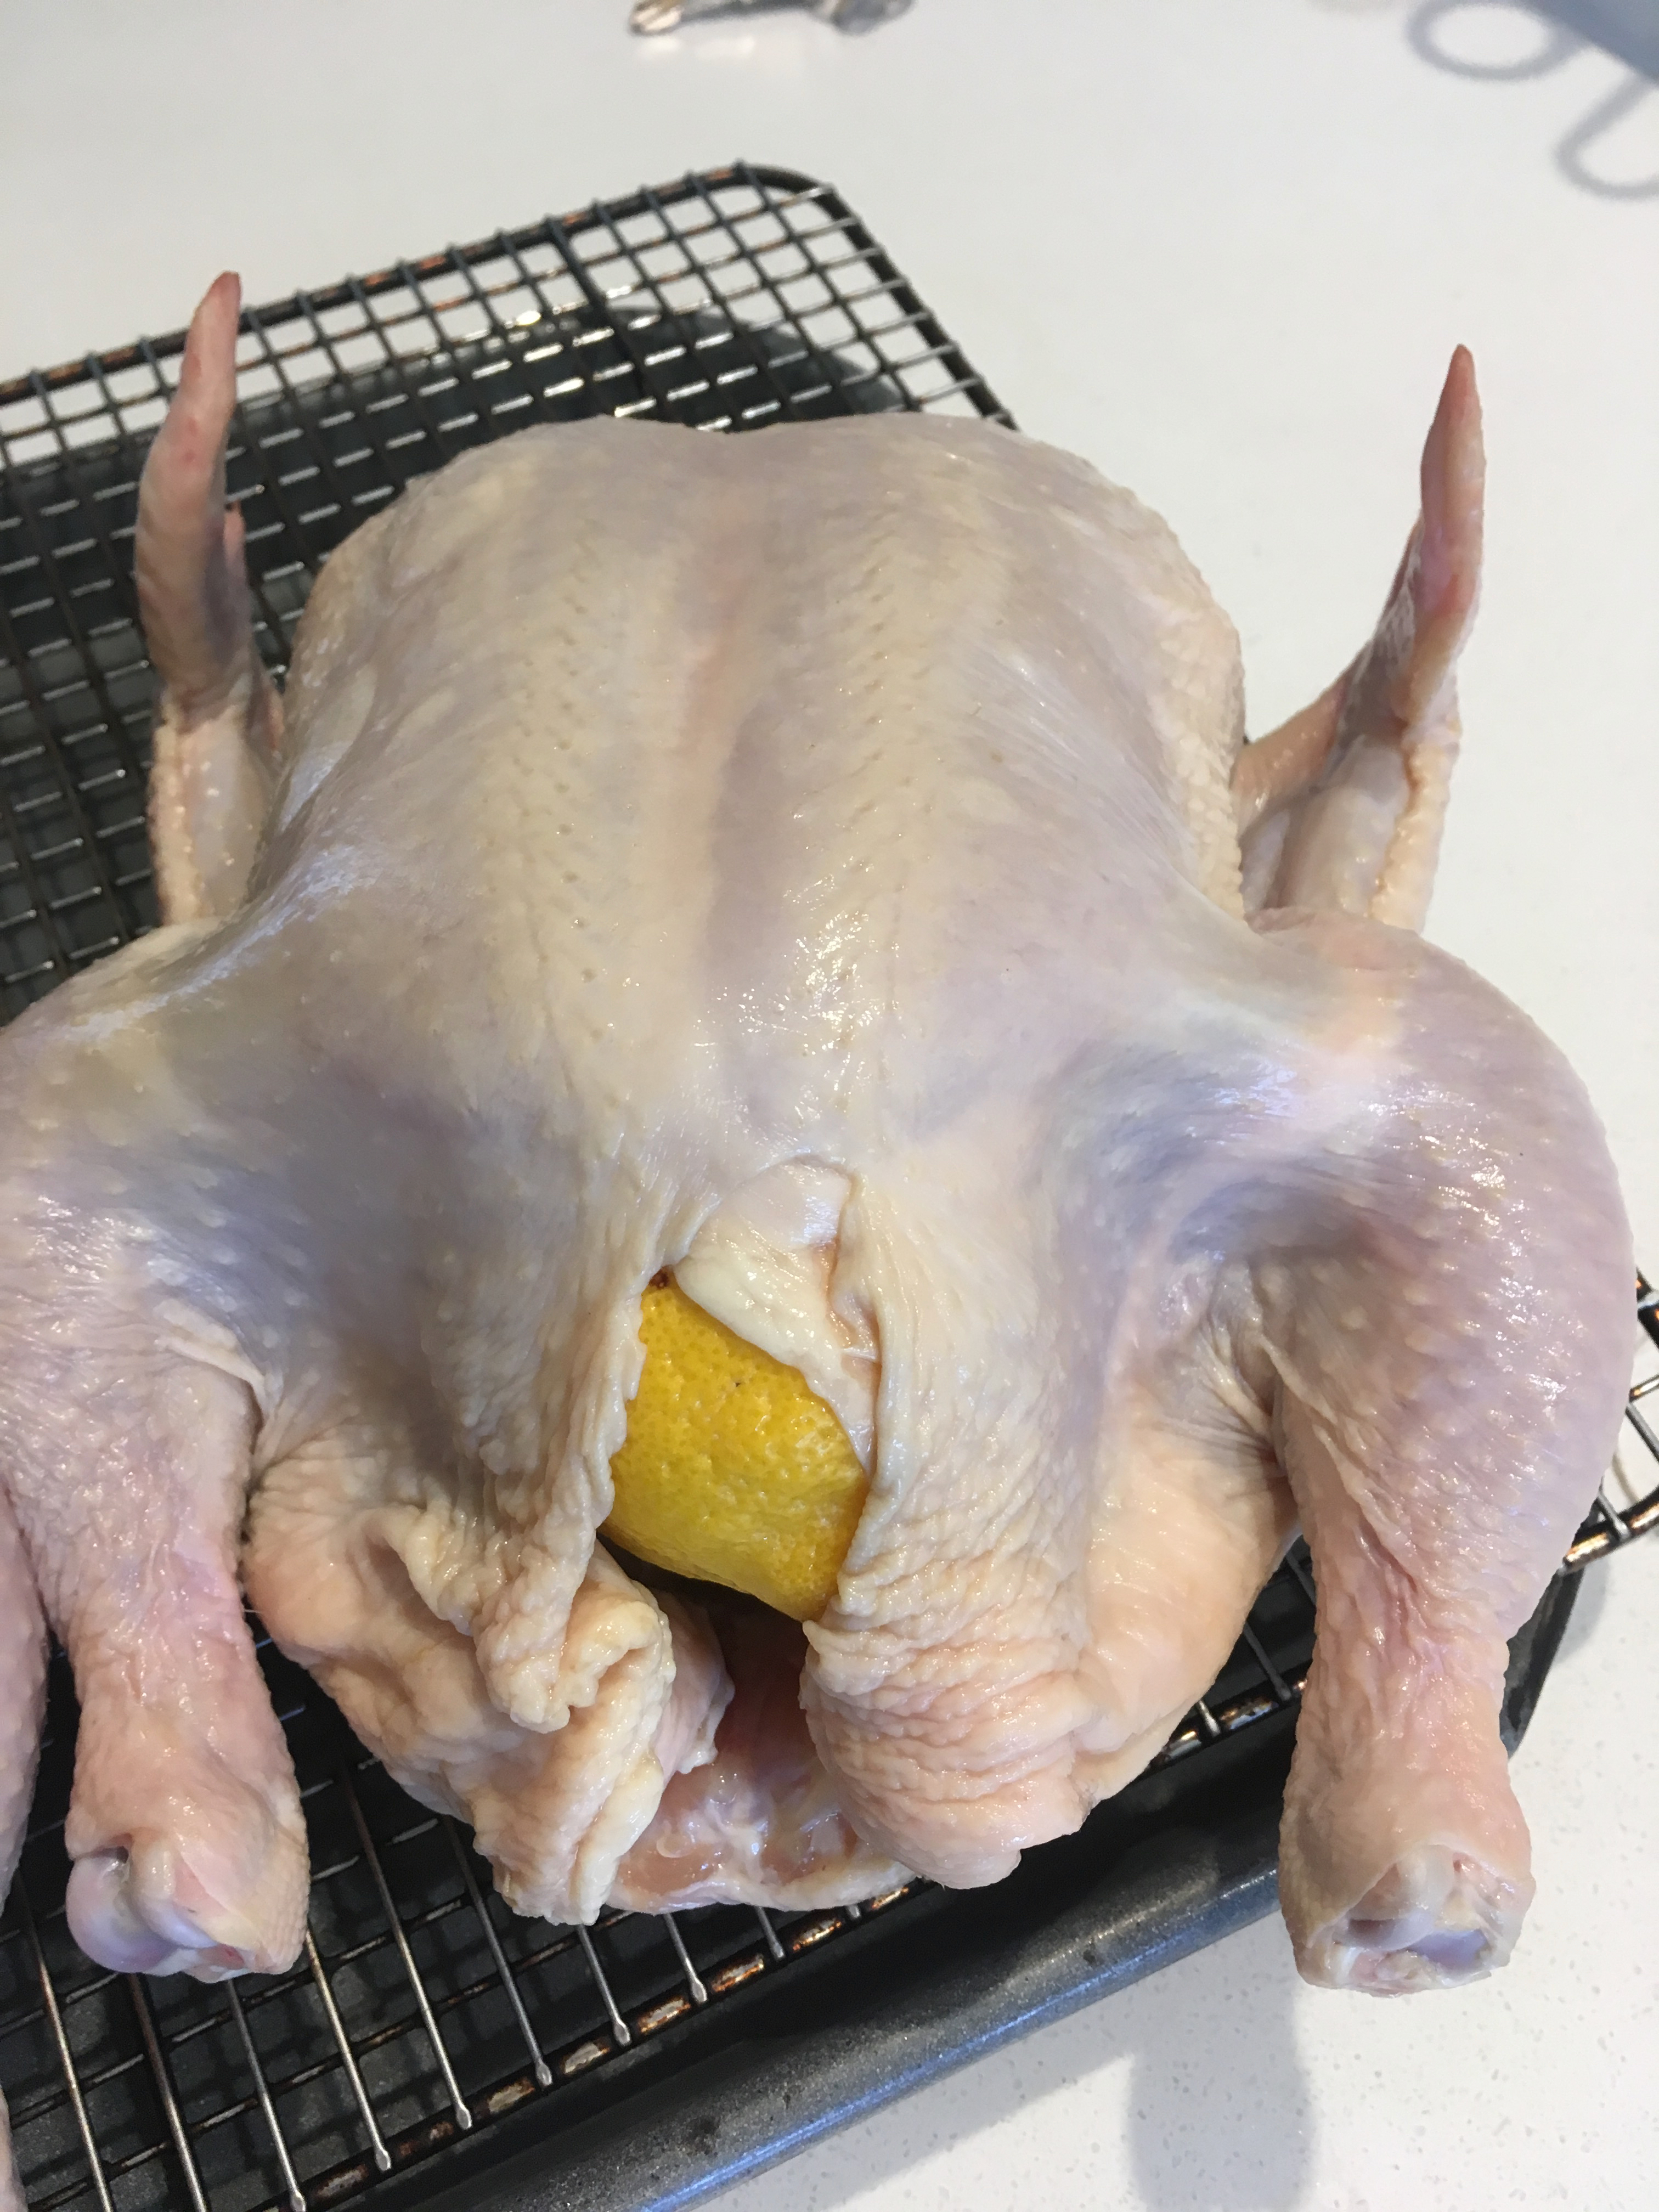
\includegraphics[width=0.25\textwidth]{\imageDir/\fileName/IMG_3213.jpg} \\
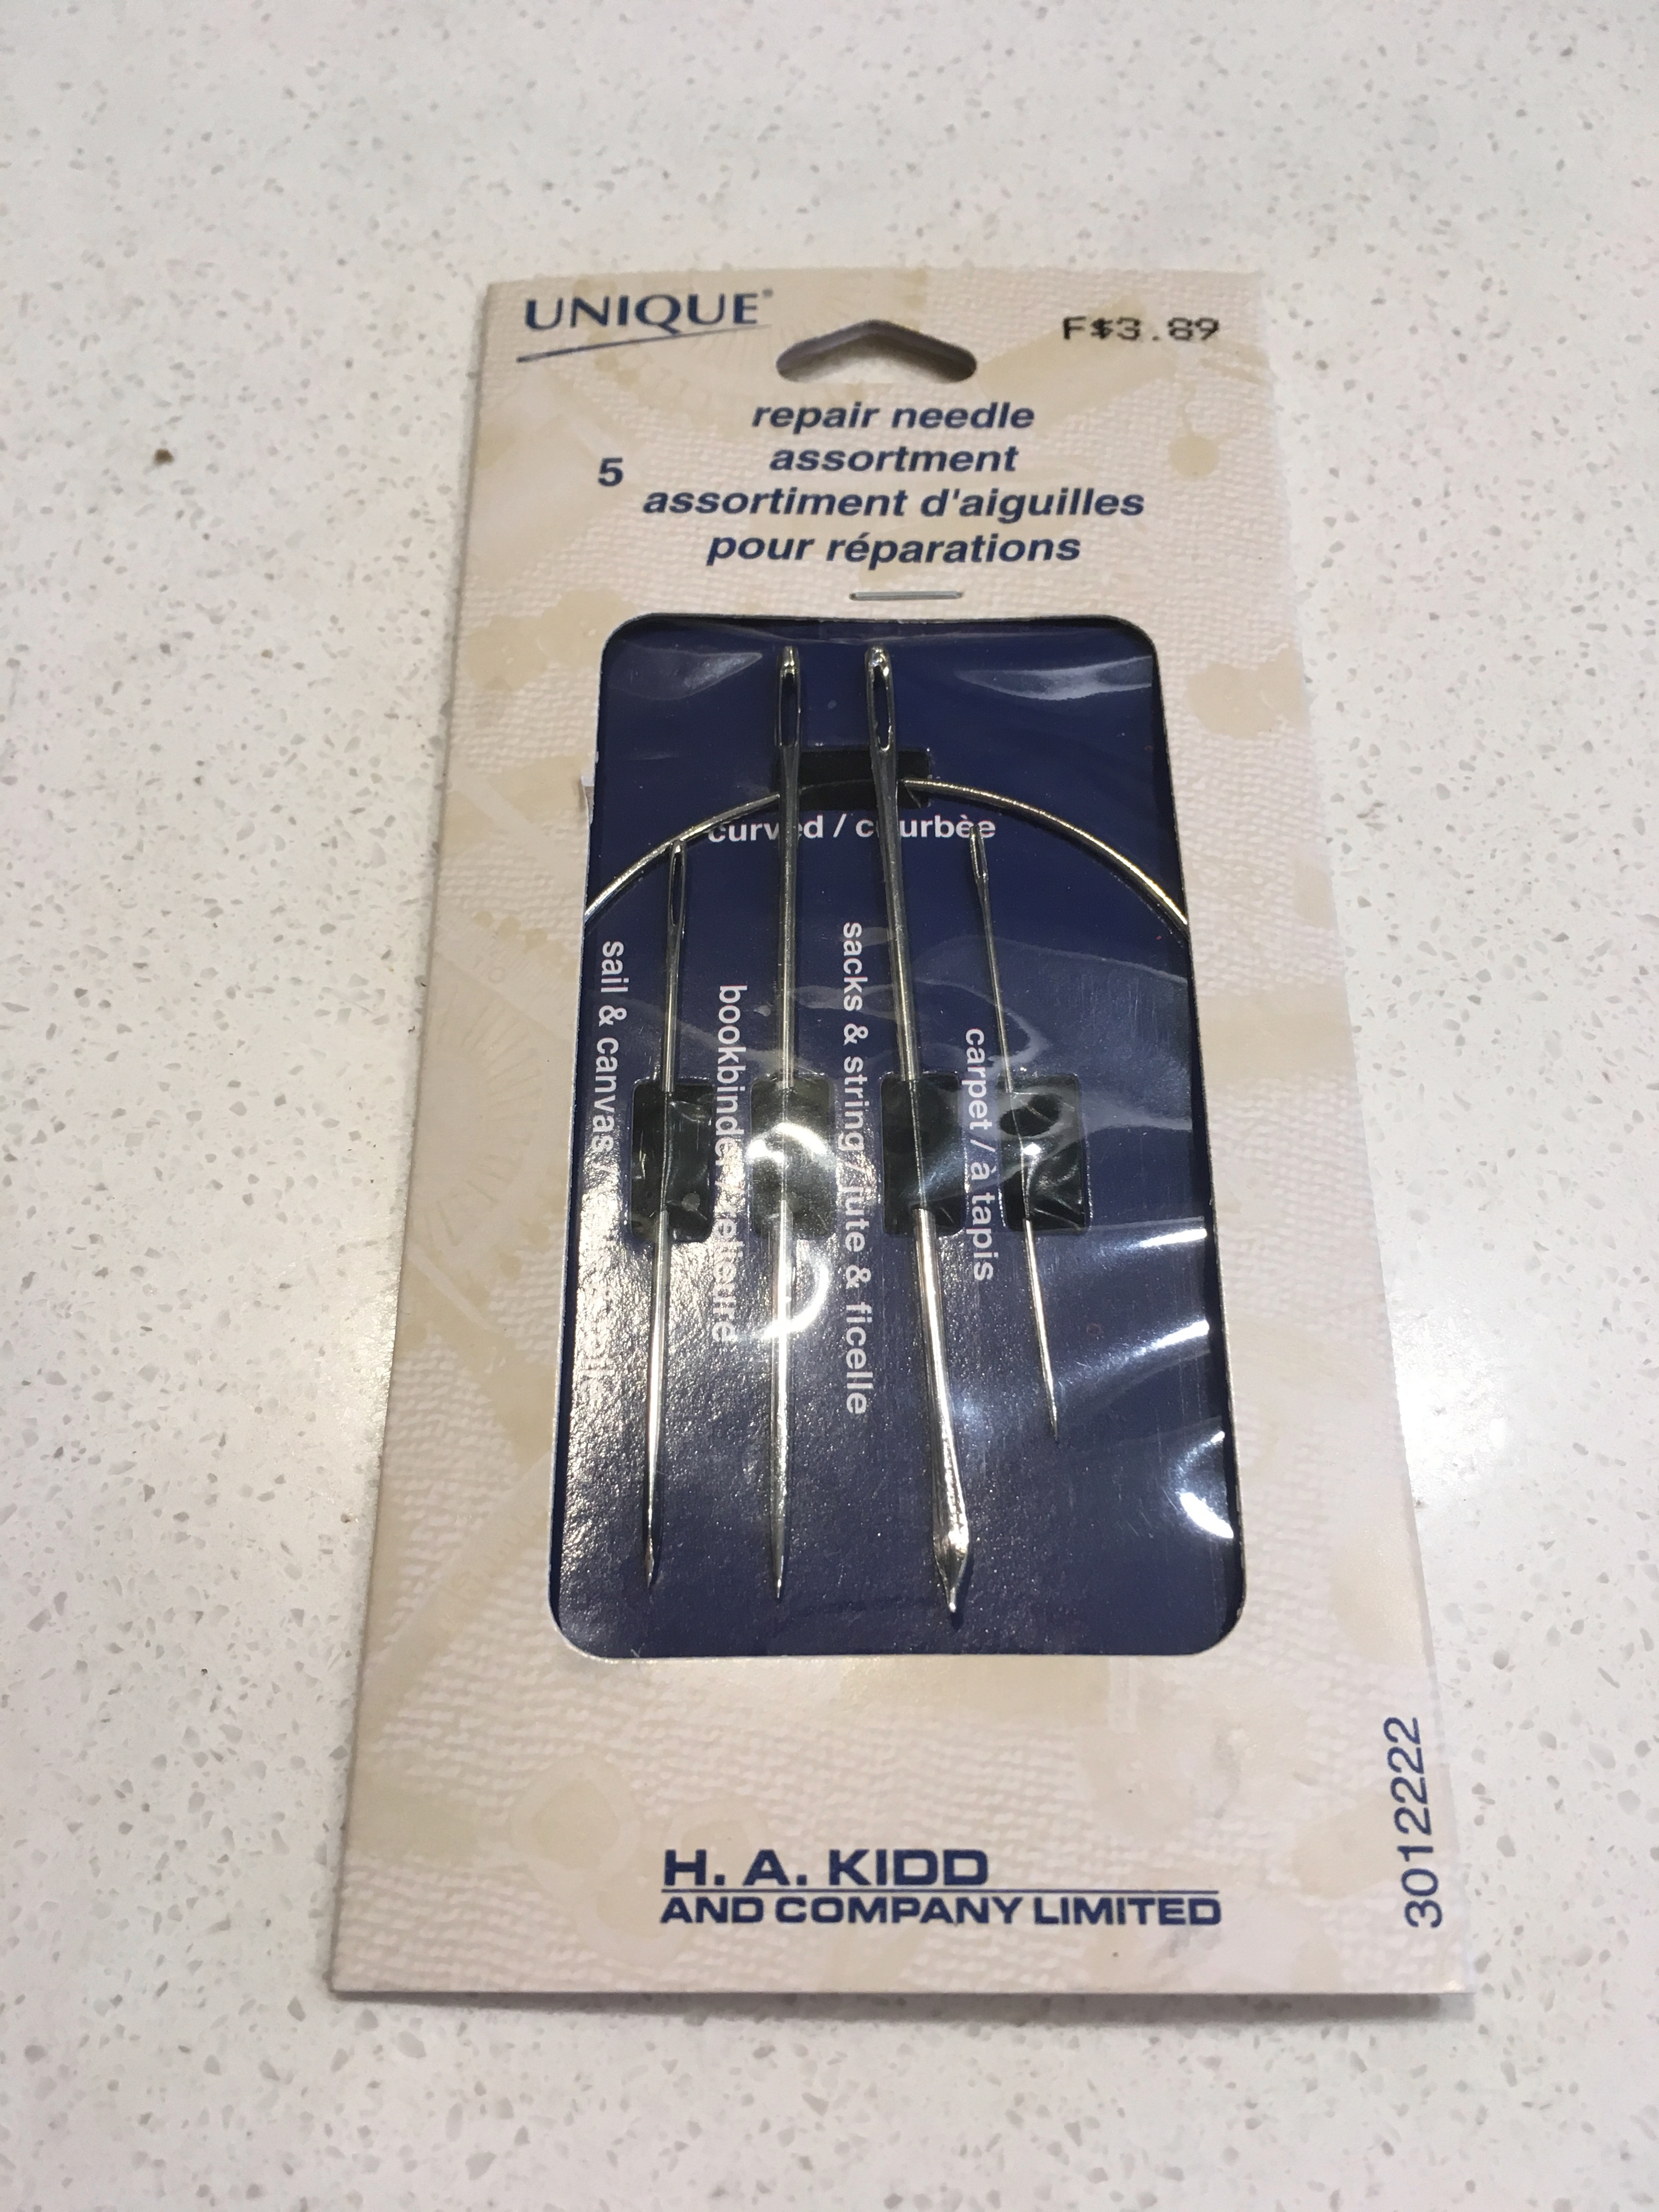
\includegraphics[width=0.25\textwidth]{\imageDir/\fileName/IMG_3206.jpg} &
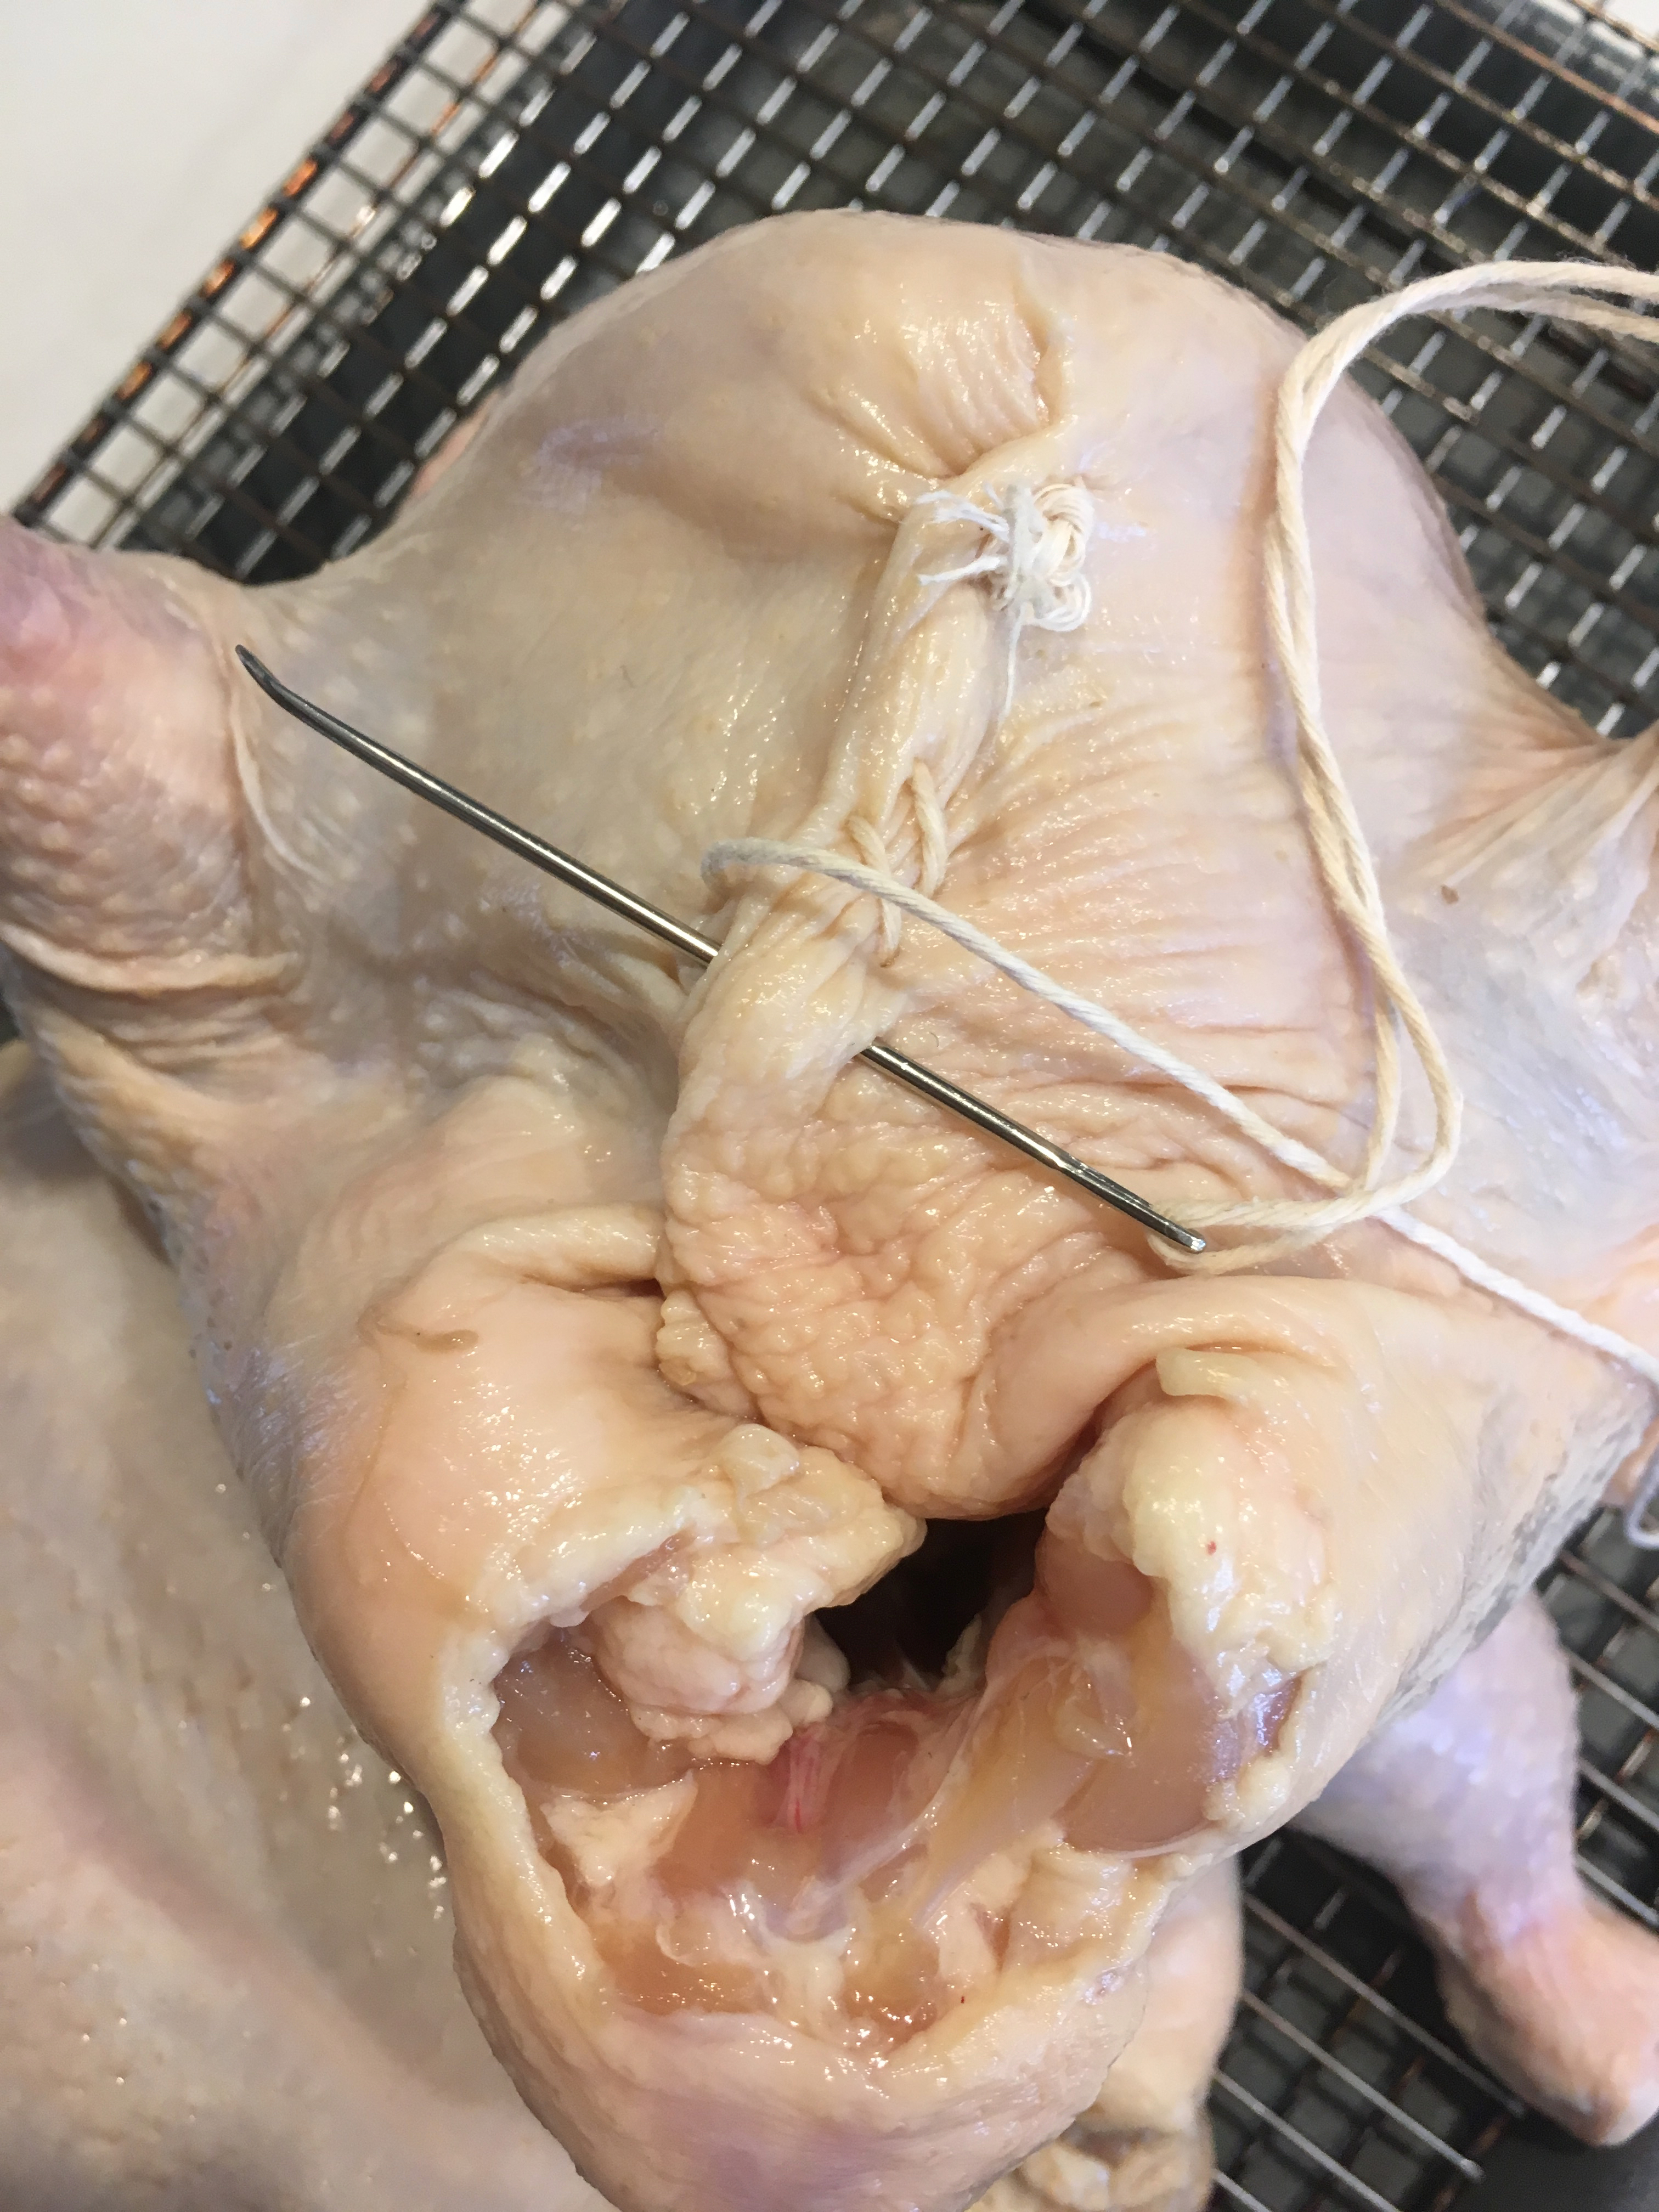
\includegraphics[width=0.25\textwidth]{\imageDir/\fileName/IMG_3214.jpg} &
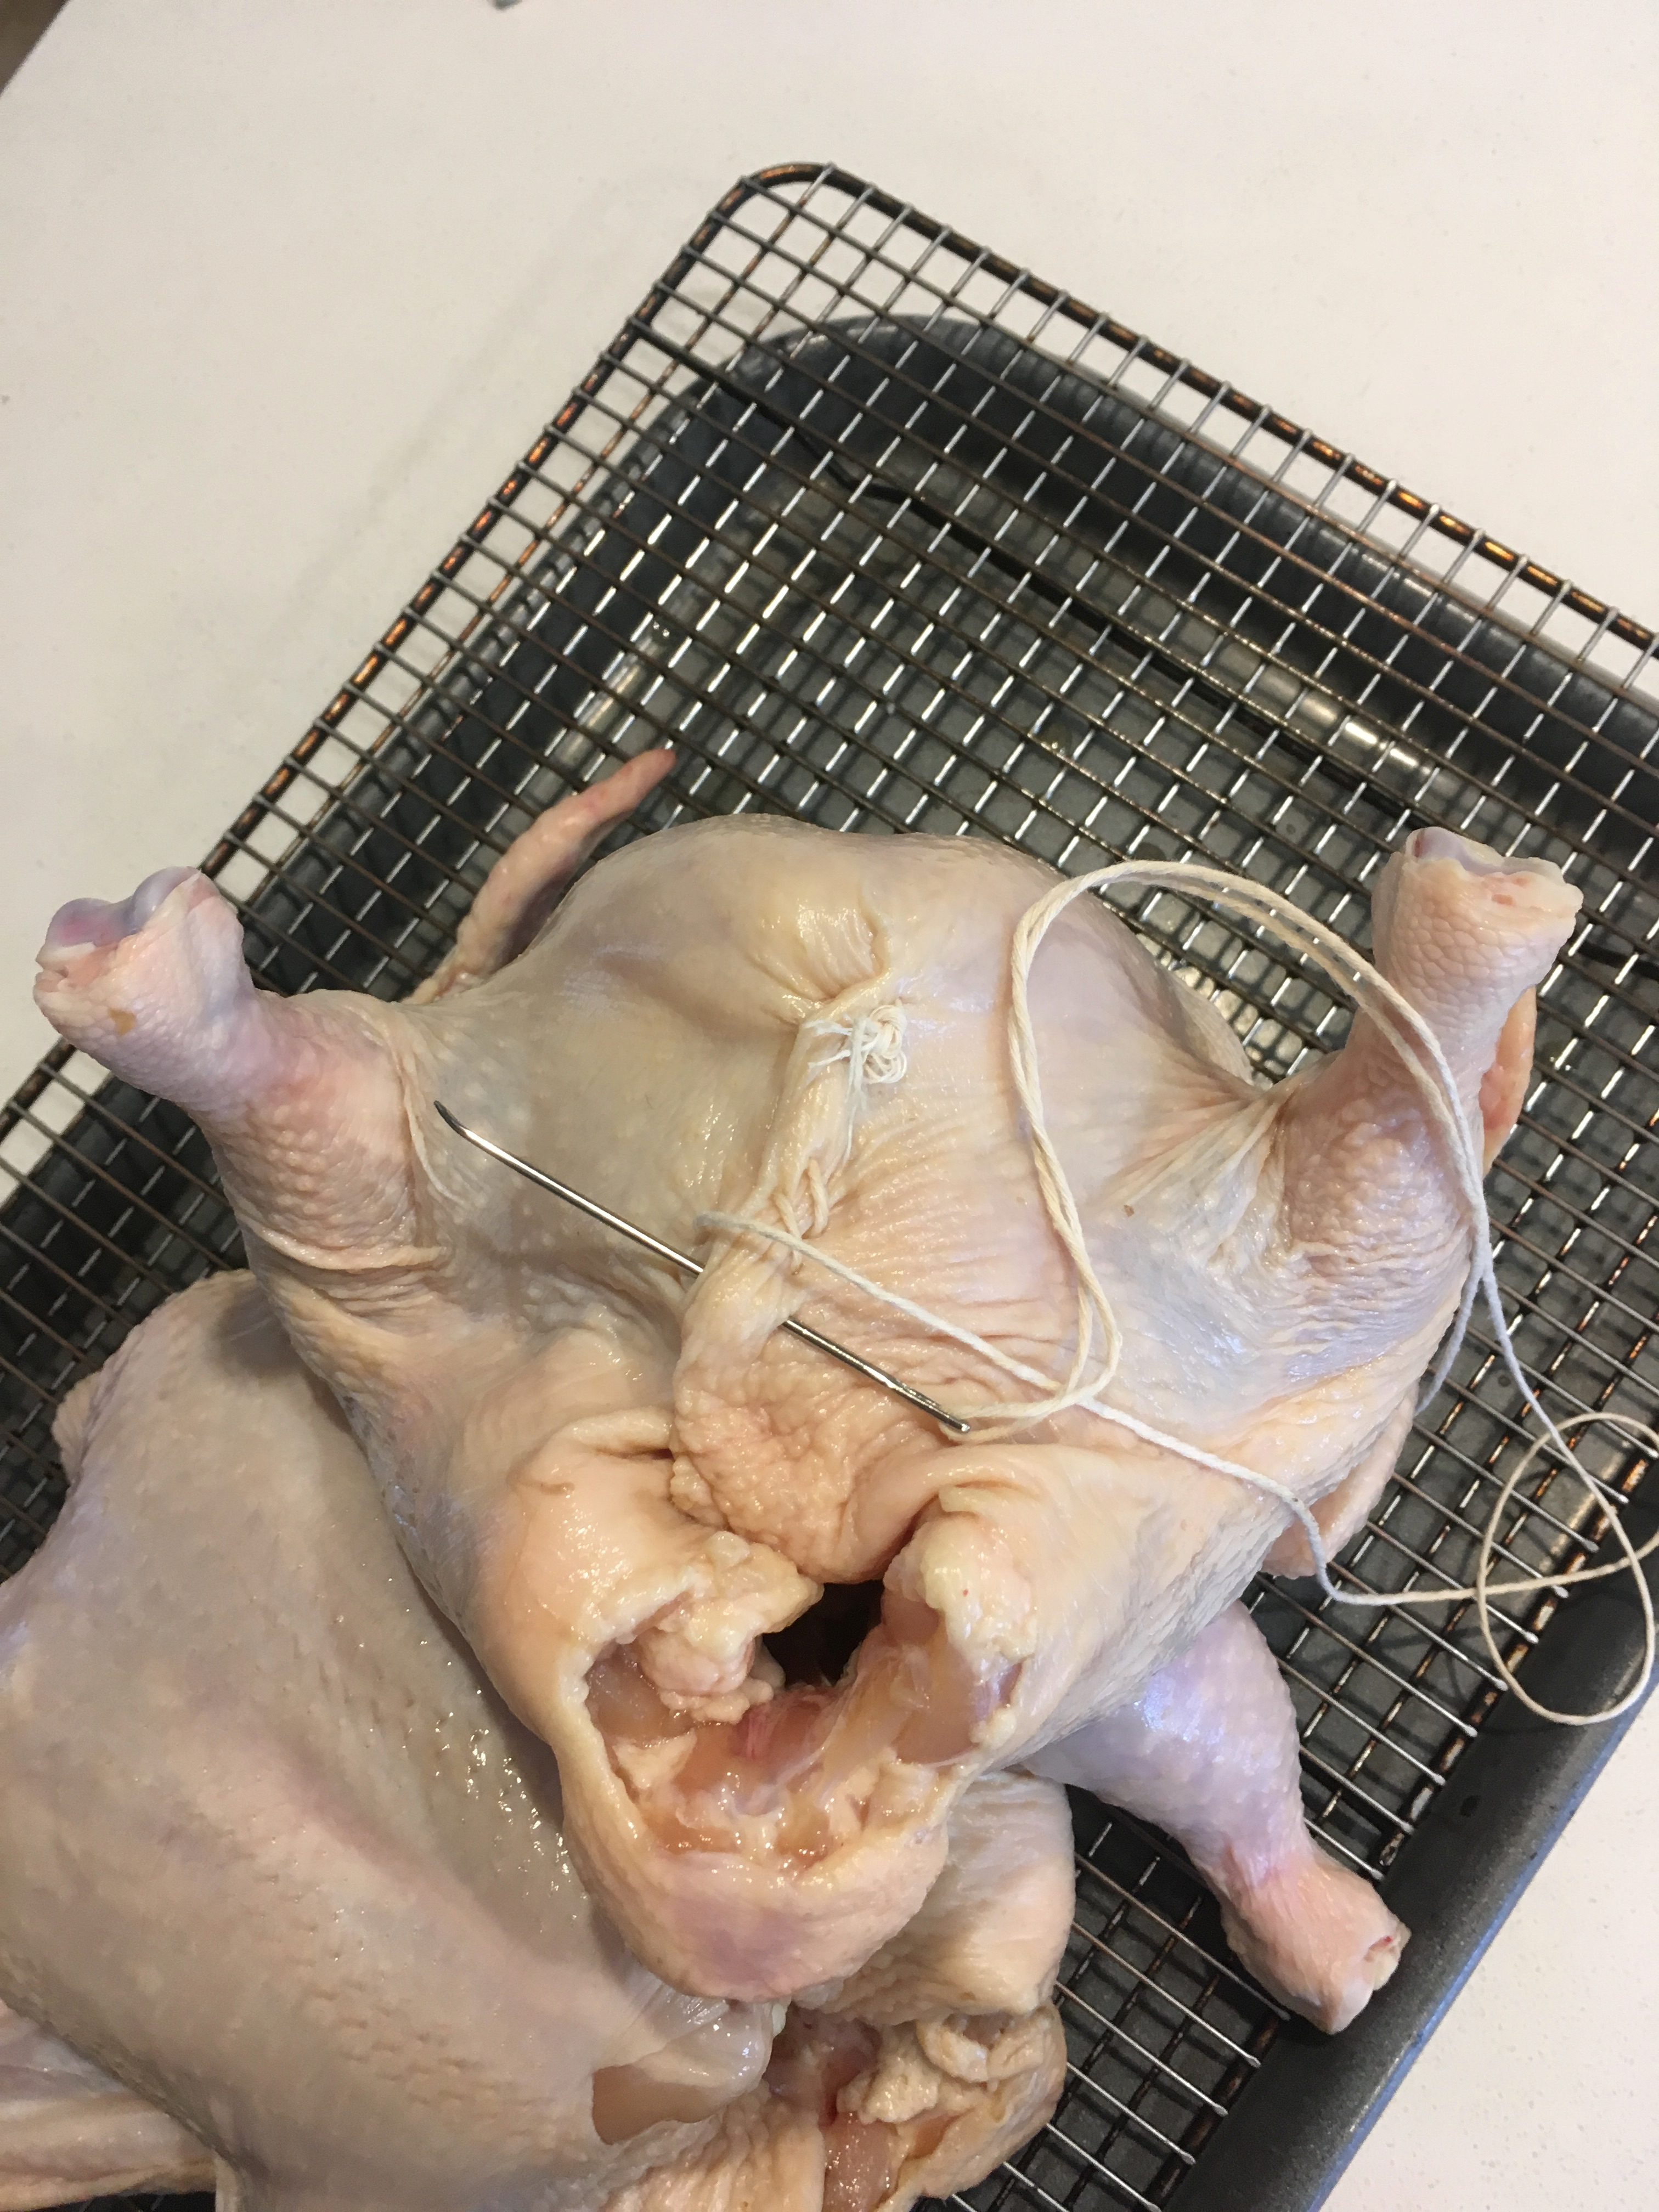
\includegraphics[width=0.25\textwidth]{\imageDir/\fileName/IMG_3216.jpg} \\
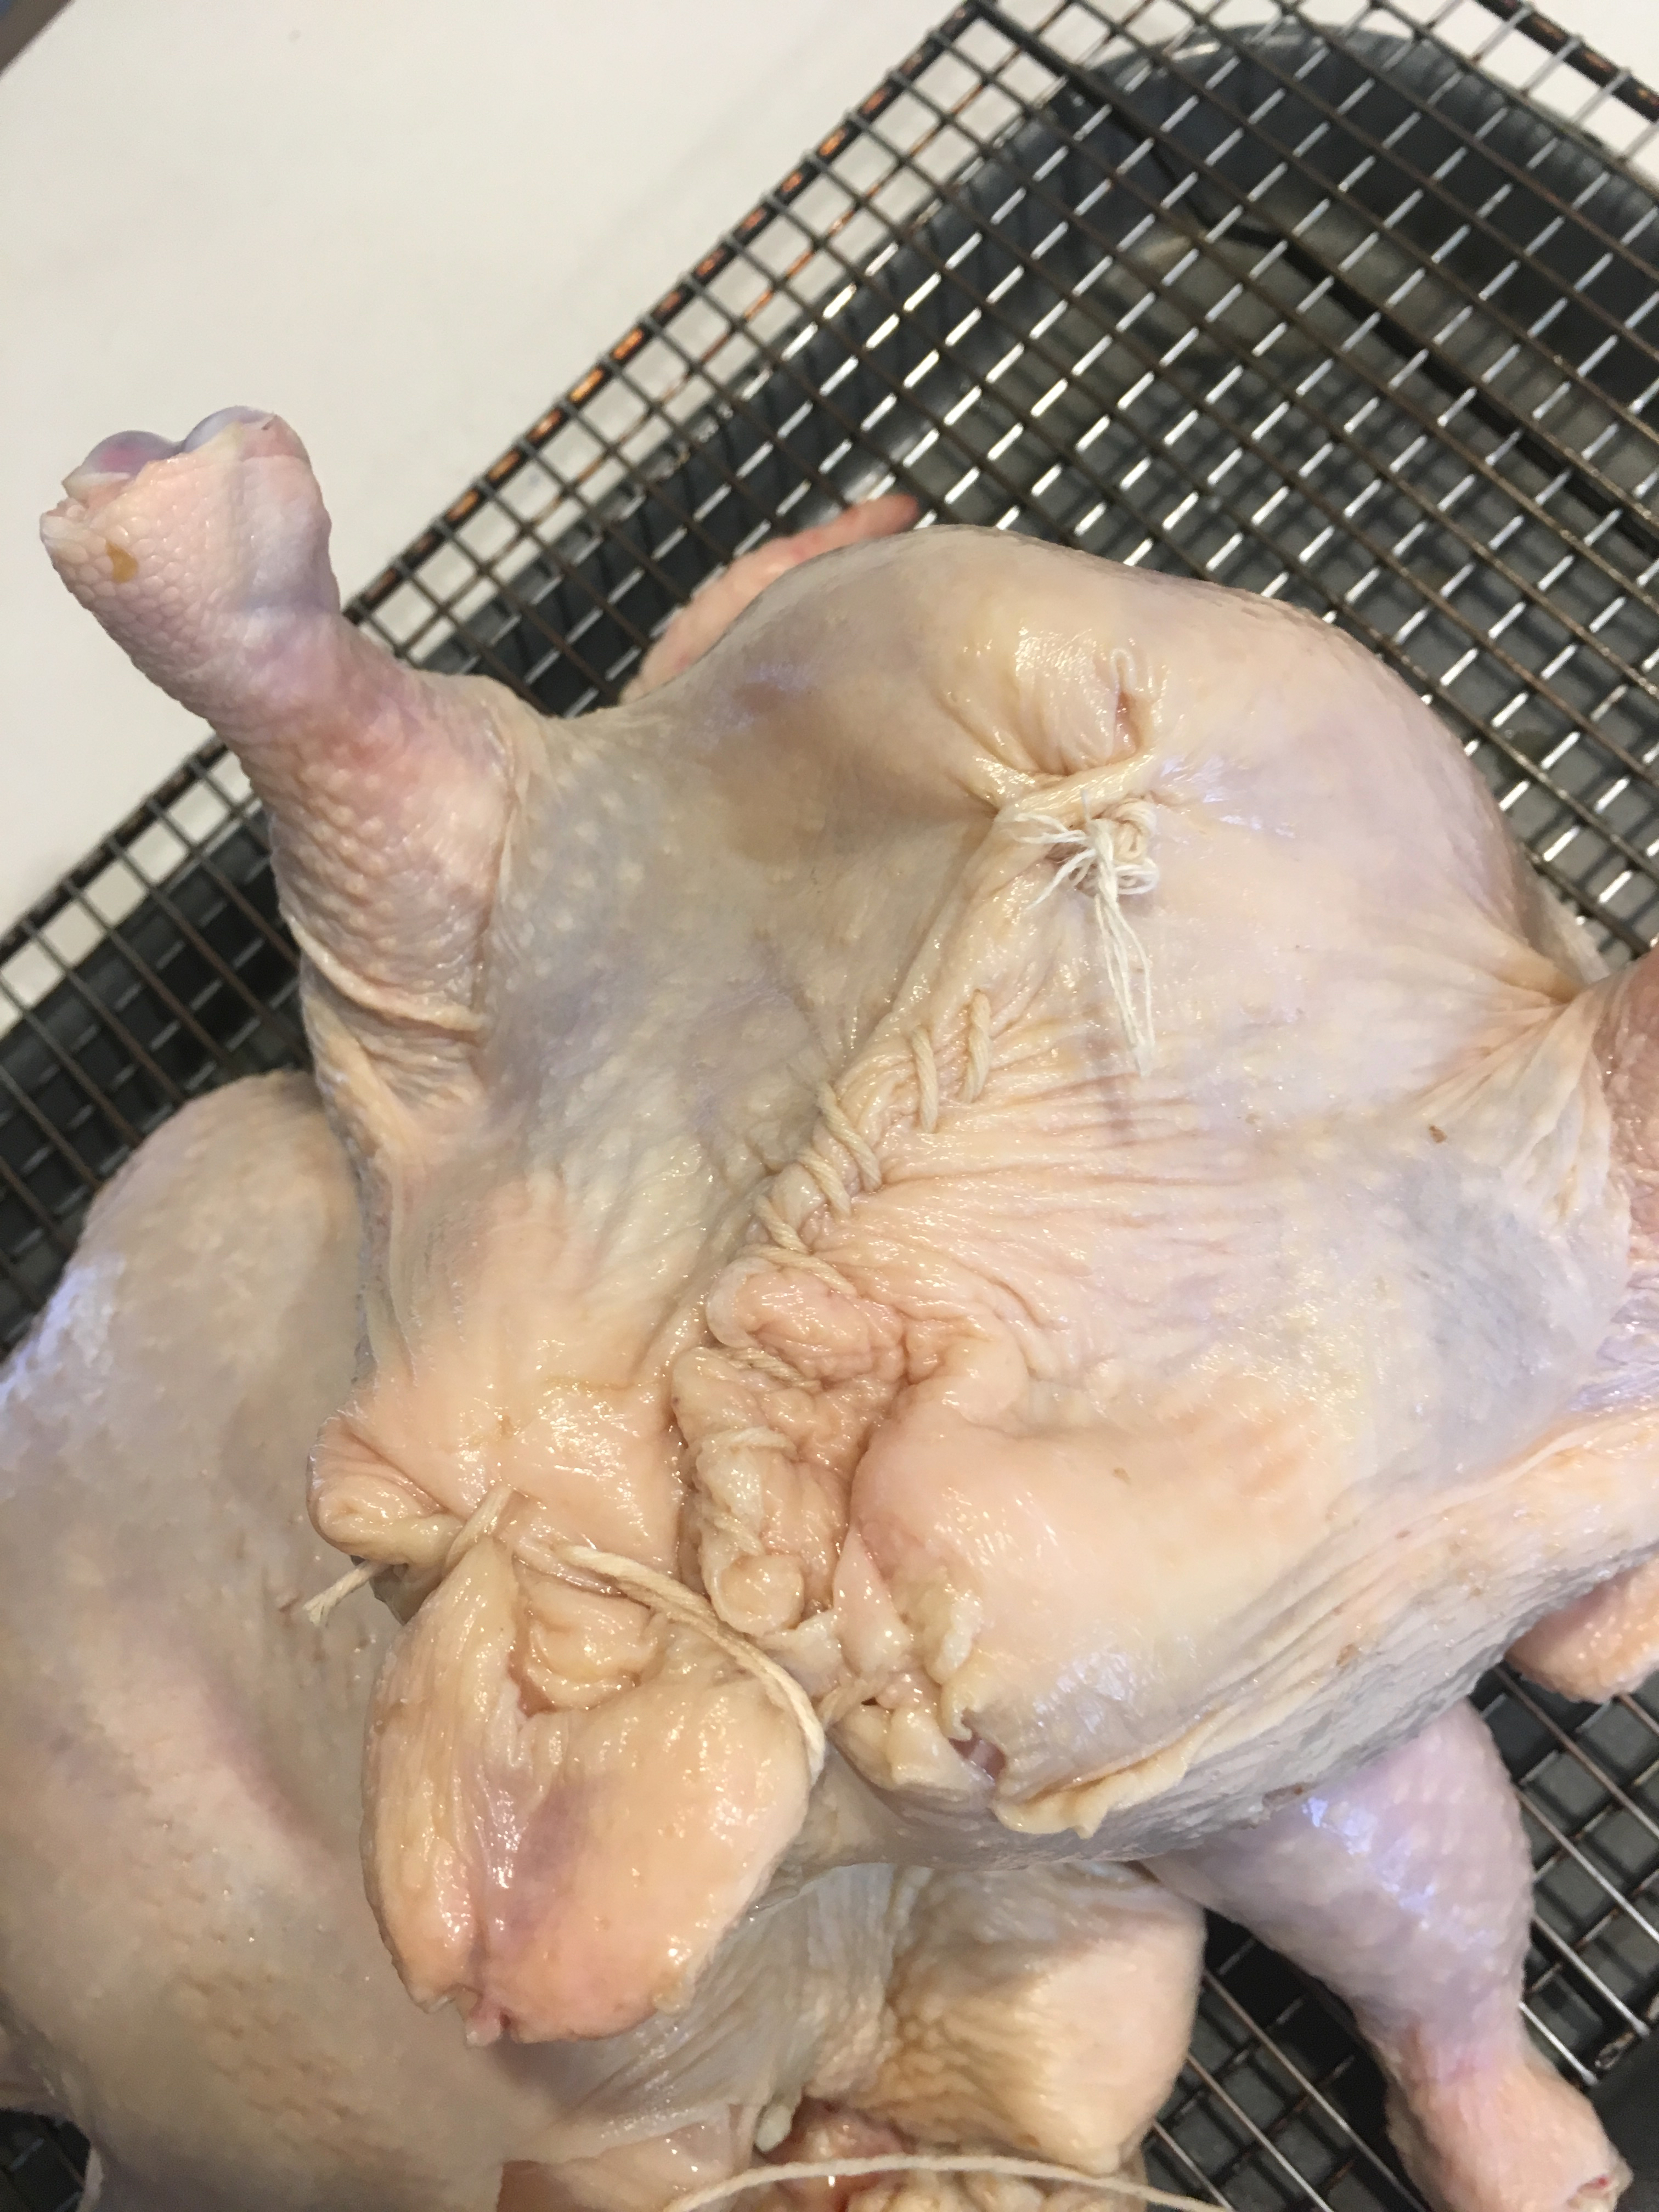
\includegraphics[width=0.25\textwidth]{\imageDir/\fileName/IMG_3217.jpg} &
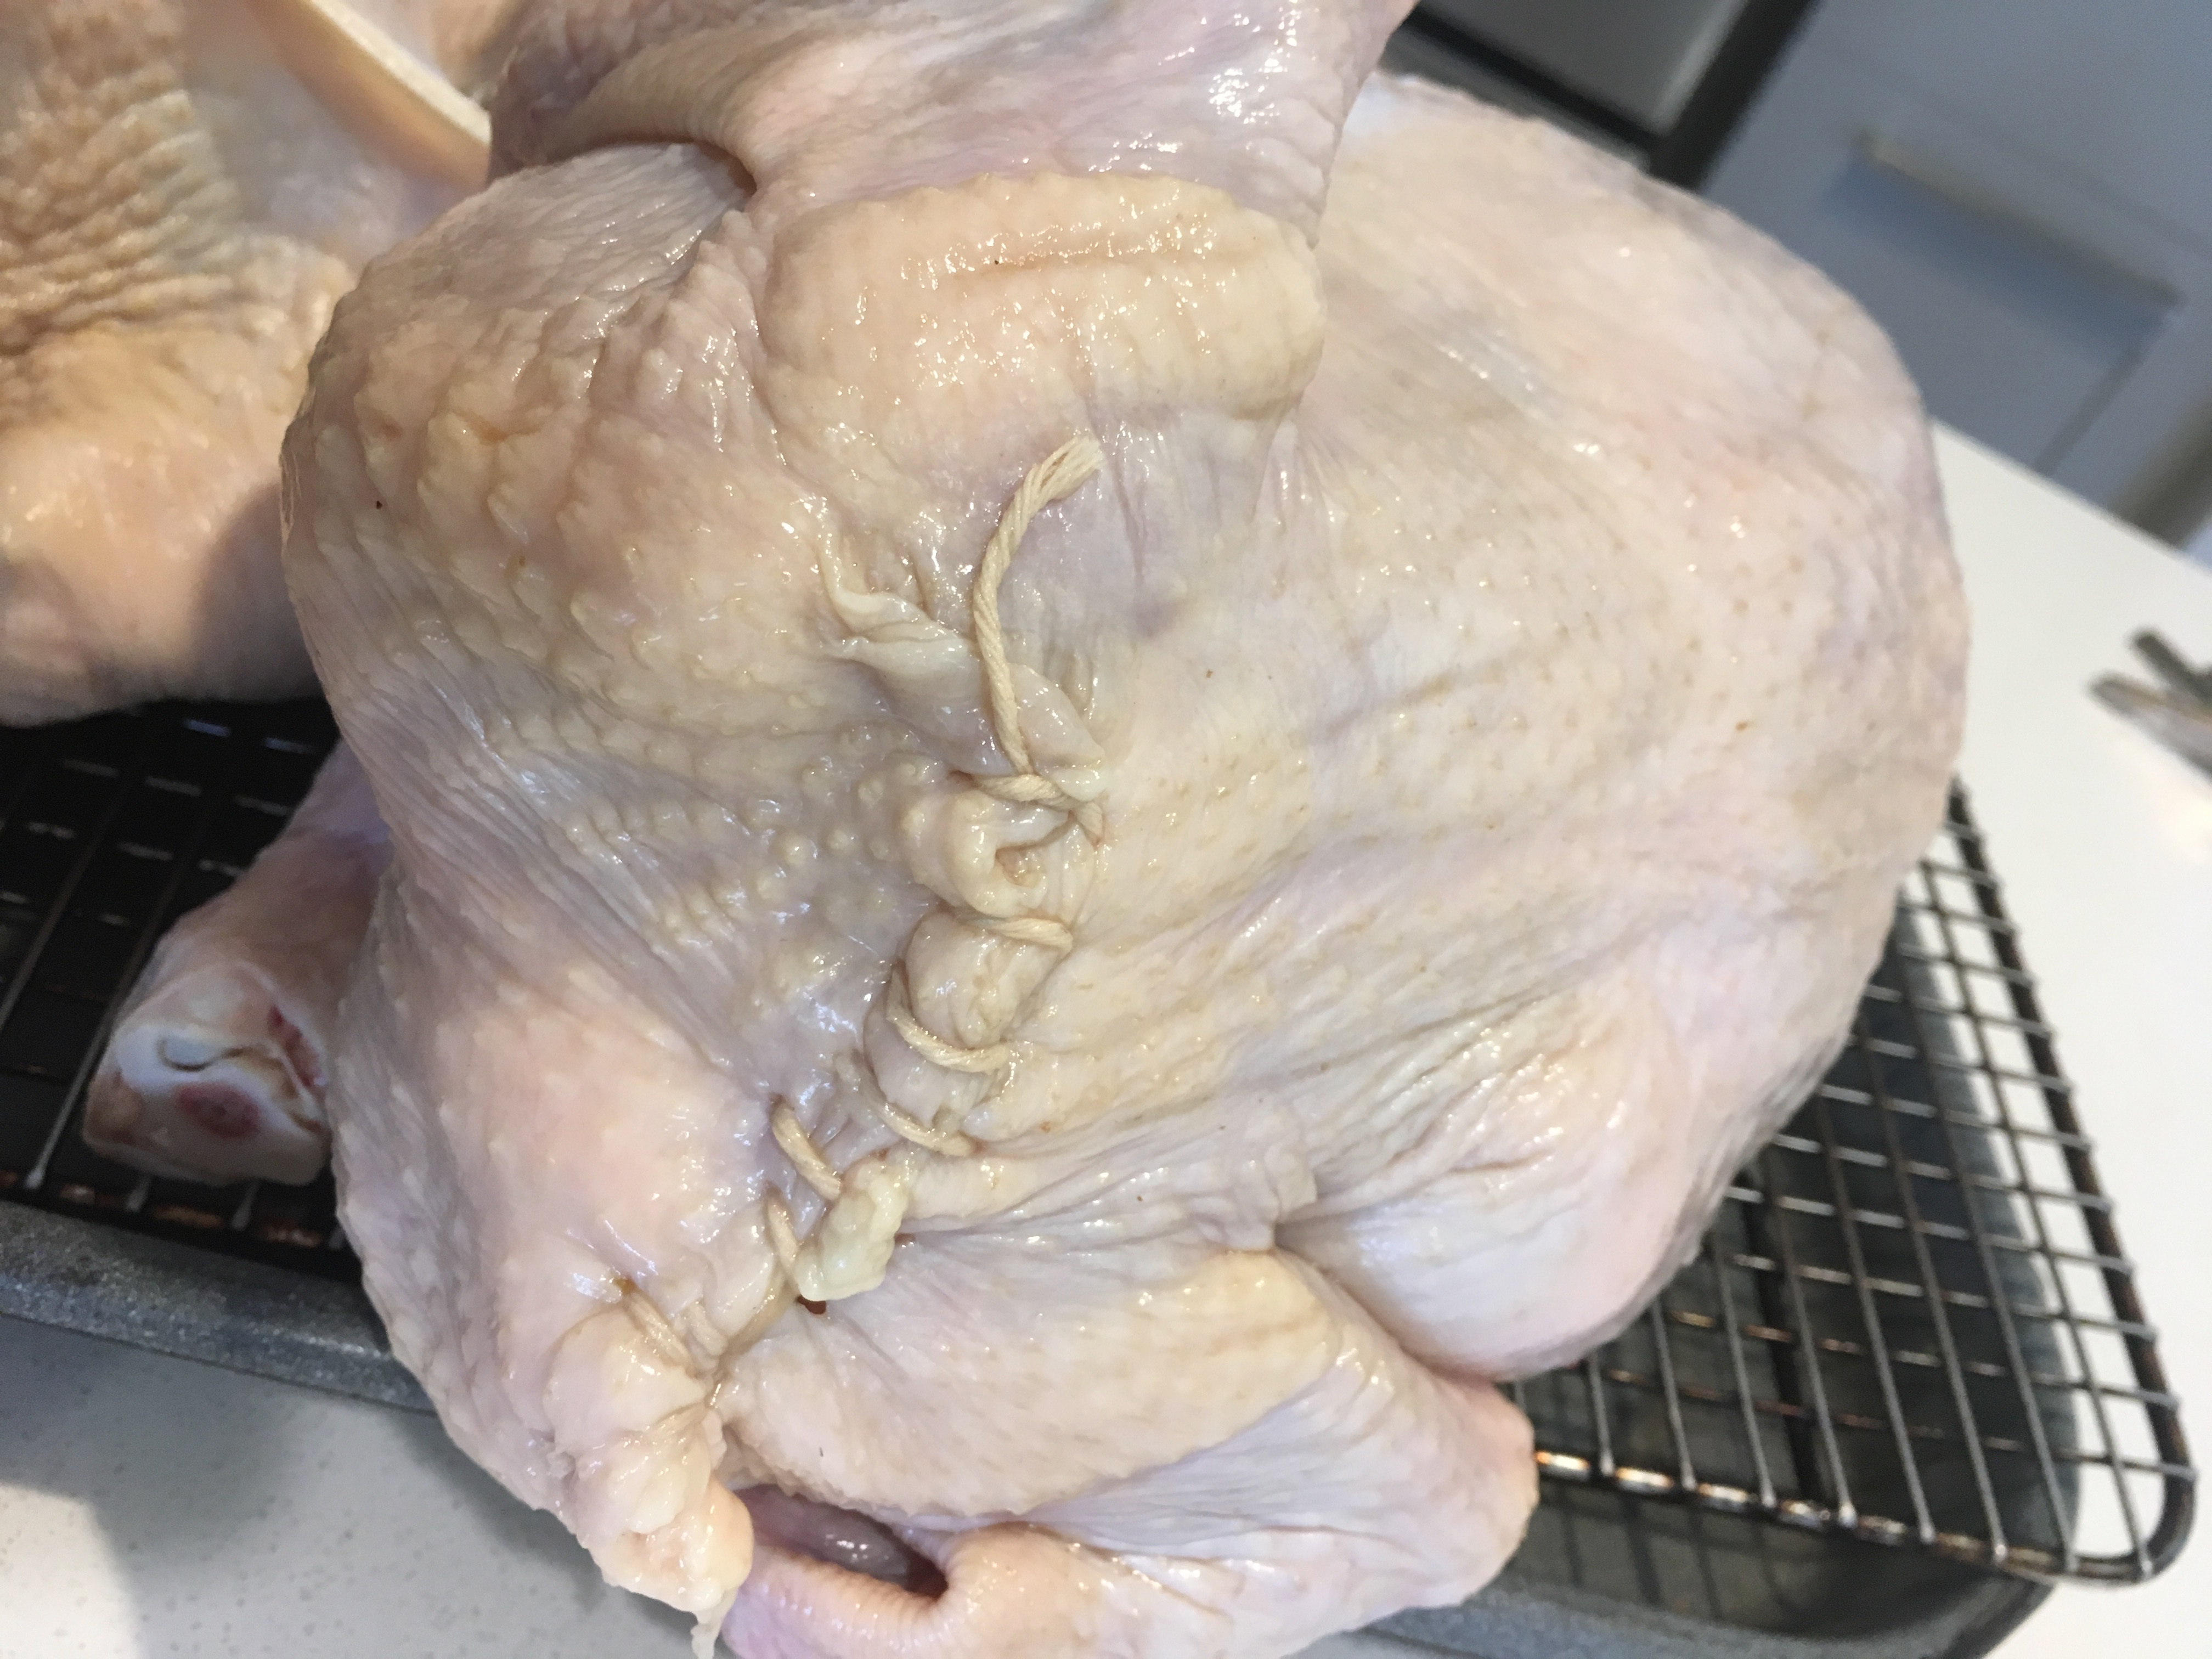
\includegraphics[width=0.25\textwidth]{\imageDir/\fileName/IMG_3218.jpg} &
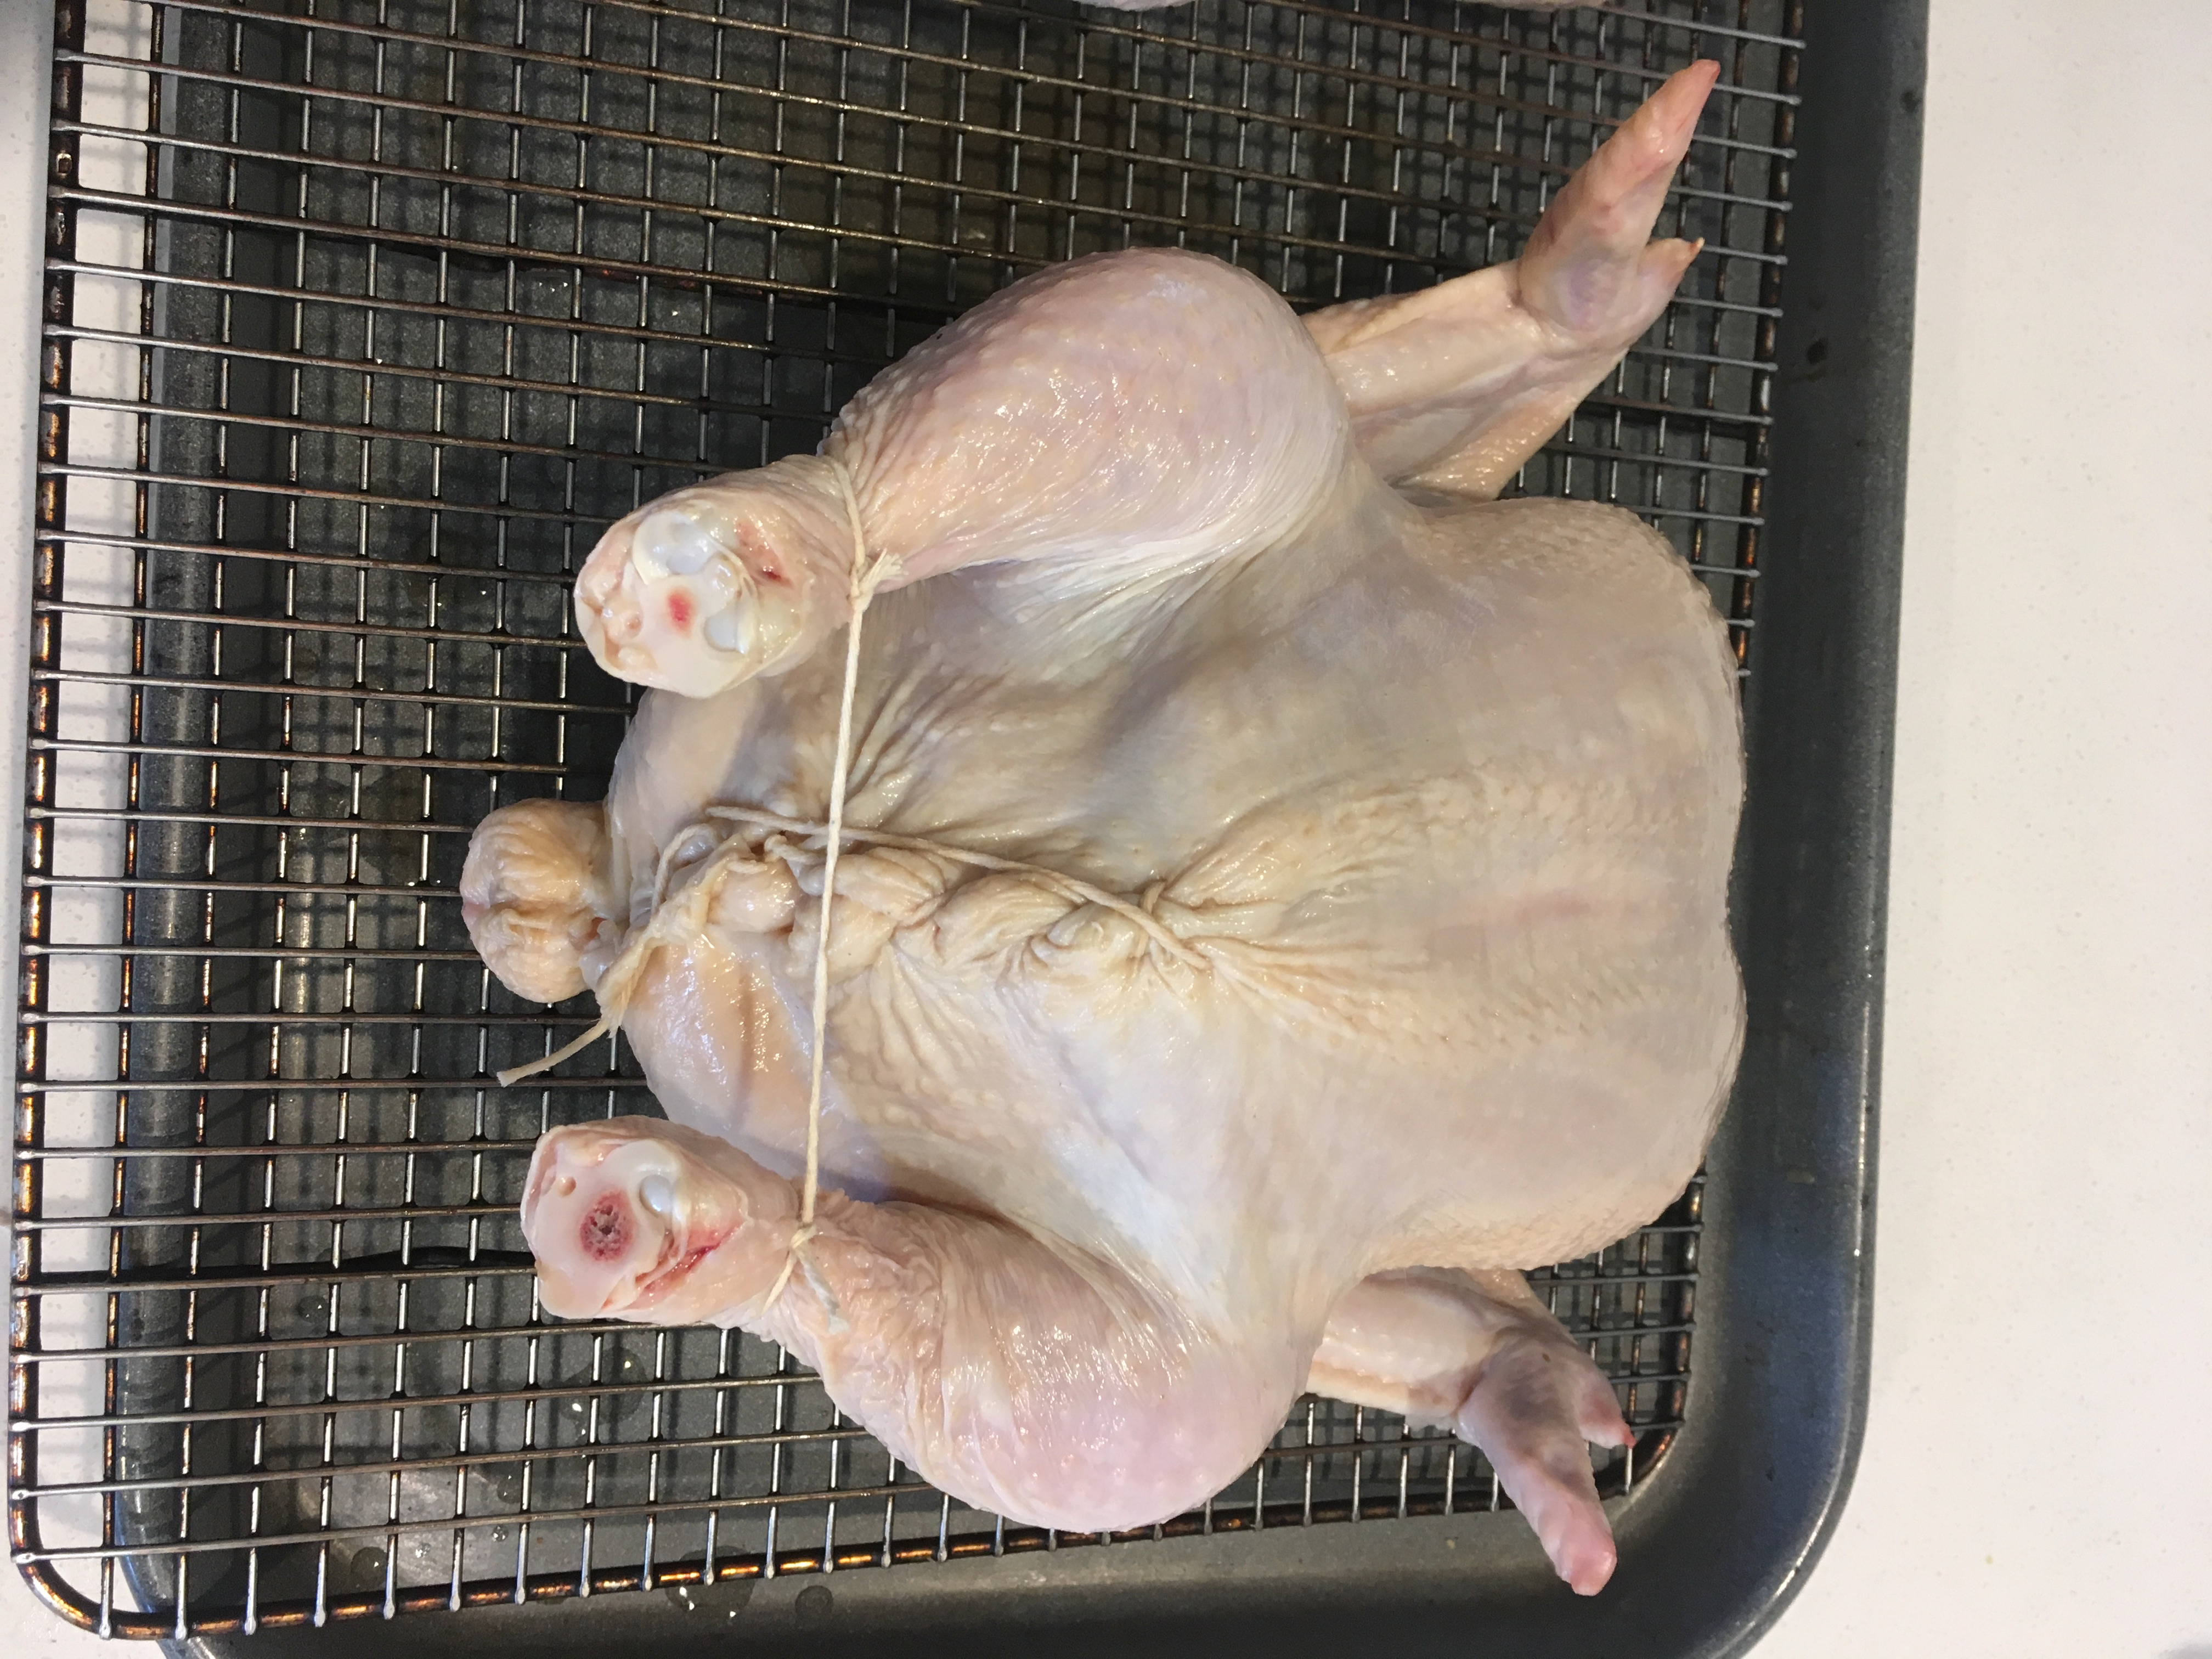
\includegraphics[width=0.25\textwidth]{\imageDir/\fileName/IMG_3219.jpg} \\
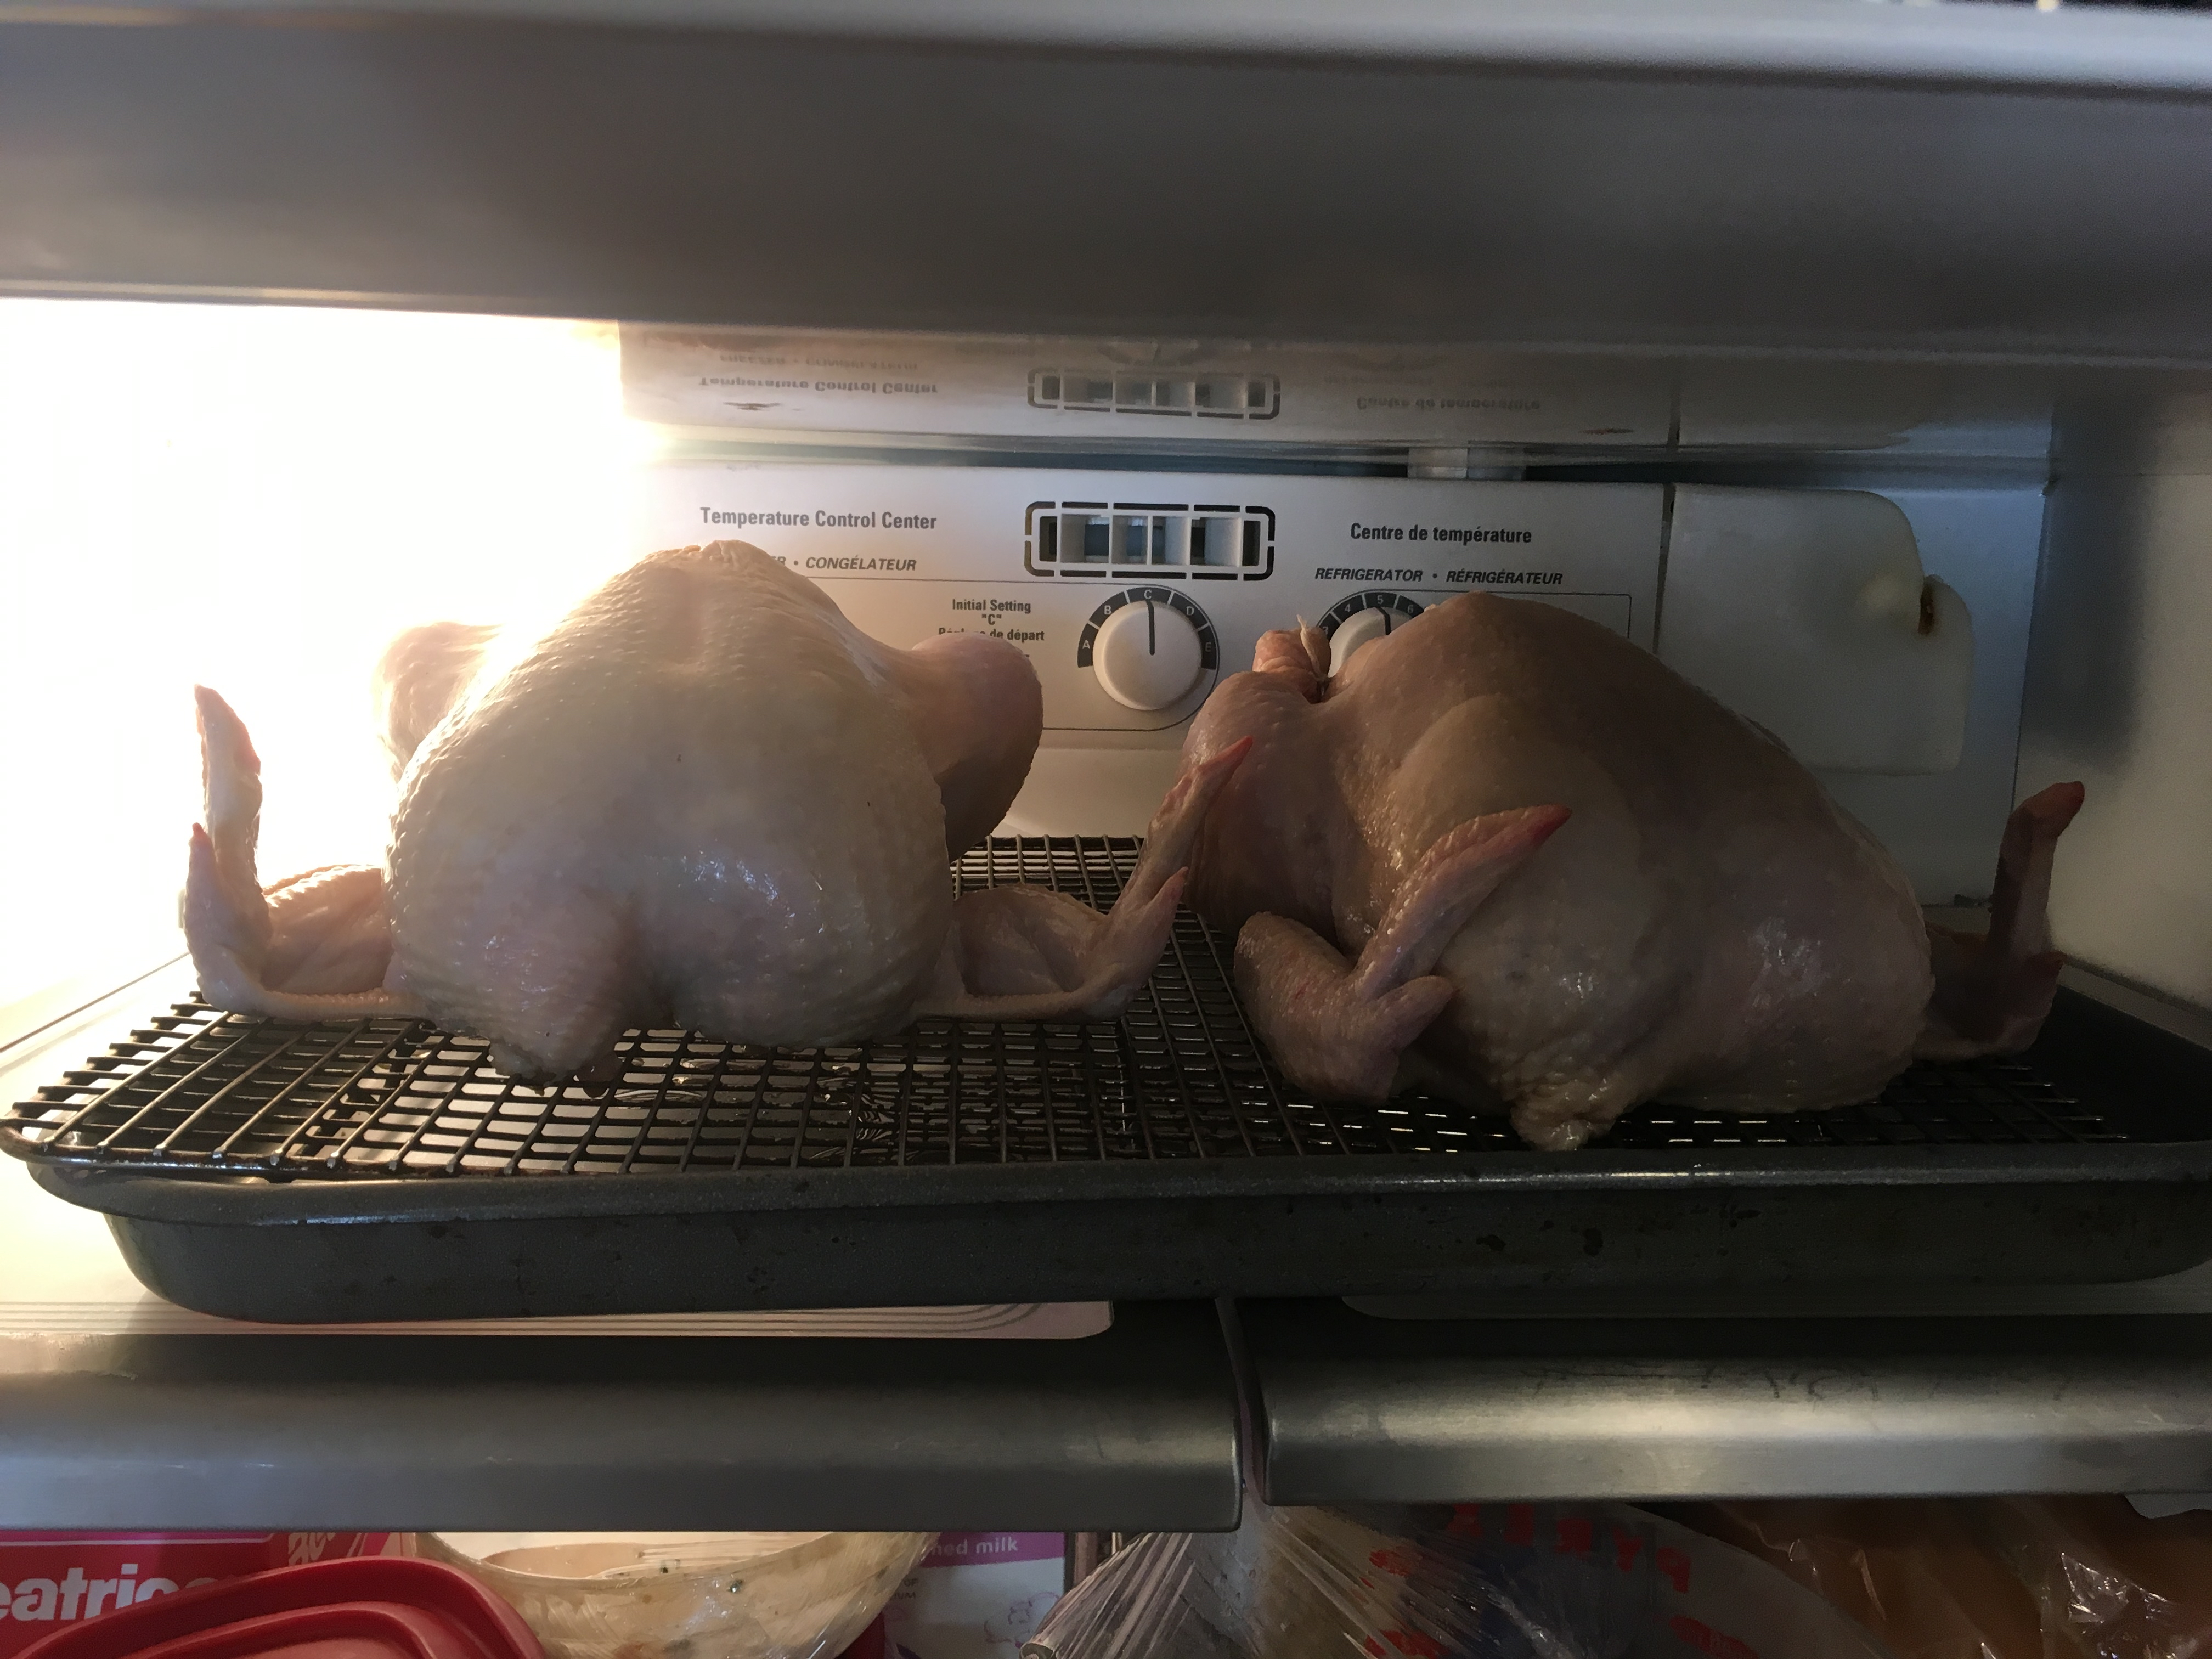
\includegraphics[width=0.25\textwidth]{\imageDir/\fileName/IMG_3220.jpg} &
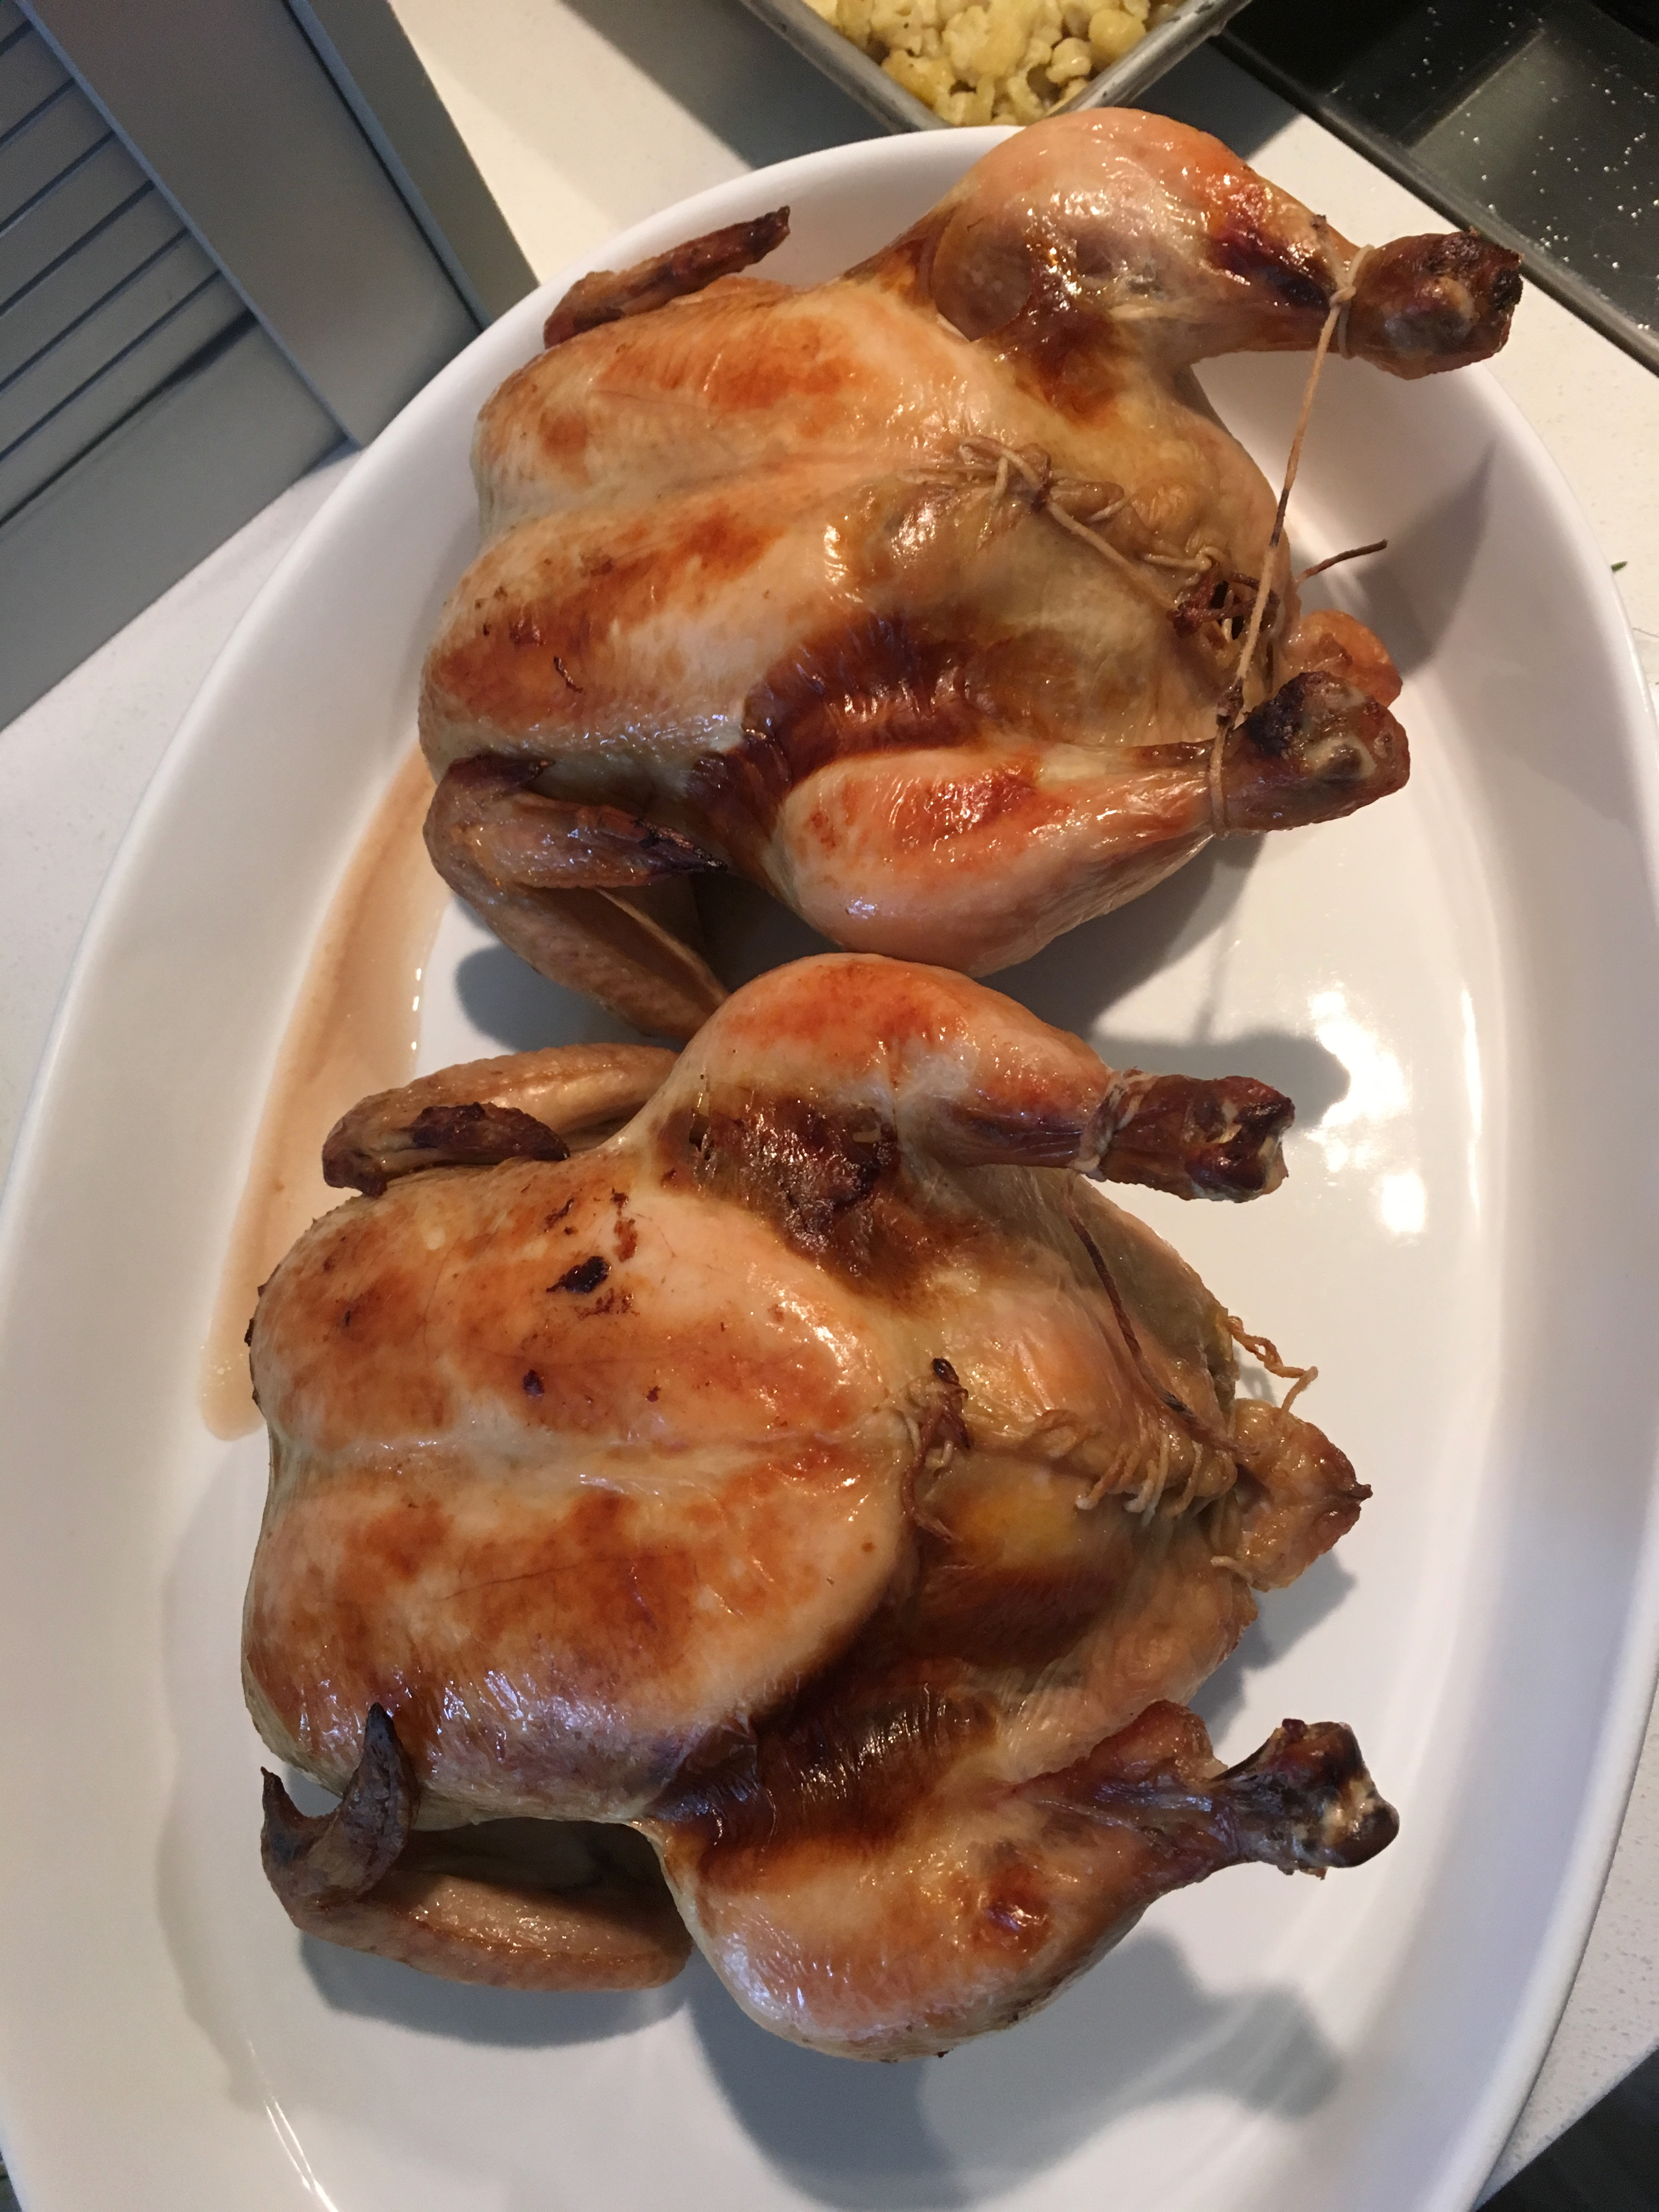
\includegraphics[width=0.25\textwidth]{\imageDir/\fileName/IMG_3228.jpg} \\
\end{tabular}
\end{table}



\end{document}
